%!TEX root = main.tex

%!TEX root = main.tex


\subsection{Semantics of $\IFAMASS$}
% In this case, we only consider the intent flags.
%To define the semantics of $\IFAMASS$, we add some auxiliary functions and predicates. 


%To define the semantics of $\IFAMASS$, we adapt slightly the notion of configurations and the auxiliary functions and predicates. 

Recall that in an  $\STK$-dominating  $\IFAMASS$, $\lmd(A) = \STD$ and $\aft(A) = \aft(A_0)$ for each activity $A$. As a result, there is only one task in each configuration and the task allocation mechanism can be ignored here. Therefore, a configuration here is simply a word $[A_1,\cdots,A_m]\in\act^+$. 
% there is only one task in $\IFAMASS$.

%Before formally defining the semantics of $\Mm$, let us first describe the intuitions of the intent flags. 
%We would like to warn that although the intuitions of these intent flags may help the readers to get some preliminary idea of their meanings, before diving directly into the formal semantics, they are nonetheless inaccurate, especially when different flags may interfere with each other.

\paragraph{Intuitions}  We explain the intuitions of the five intent flags. 
\begin{itemize}
	\item $\stpflag$:  If it is set,  it has the same effect as starting an activity of the $\STP$ launch mode.
	\item $\ctpflag$:  If it is set, it will check for the existence of the started activity in the task. If the activity exists, then all the activities above the topmost occurrence of the started activity in the task will be removed. Otherwise, the started activity will be pushed into the task.
	\item $\rtfflag$:  If it is set, it will check for the existence of the started activity in the task. If the activity exists, then the topmost occurrence of this activity will be moved to the top of this task. Otherwise, the started activity will be pushed into the task.
	\item $\ntkflag$:  If it is set, it will look for an existing task to put the started activity according to the task allocation mechanism. If such a task exists, the task will be moved to the top and the started activity is pushed to the task, otherwise a new task is created to put this activity.
	\item $\ctkflag$: It is usually used together with $\ntkflag$. If it is set, it will remove all the activities in the task and push the started activity to the task.
\end{itemize}
%Moreover, $\ntkflag$ will only affect $\ctkflag$ in $\IFAMASS$, since there is only one task in $\IFAMASS$, task allocation mechanism will always allocate the top task.

%To define the semantics of $\IFAMASS$, the concept of configuration is adapted from the definition of configuration for $\LMAMASS$ as follows: A configuration of $\Mm$ is encoded as $[A_1,\cdots,A_m]\in\act^+$.

%Then we introduce some additional and adapted auxiliary functions and predicates that are to be used in the formal semantics of $\IFAMASS$.\\
We repeat the \textbf{Caveat} in Section~\ref{sect:semlmamass} for the intuition and introduce some additional functions and predicates. 
%\emph{Auxiliary functions and predicates.} 
For the configuration $\rho = [A_1,\cdots,A_m]$, 
%We define the following auxiliary functions and predicates.
\begin{itemize}
	% \item $\topact(\rho) = A_1$, $\btmact(\rho) = A_m$,
	%	\item $\push(\rho, B) = [B, A_1,\cdots,A_m]$,
	%	\item $\Pop(\rho) = [A_2,\cdots,A_m]$,
	% \item $\mvacttop(\rho, B) = ([B]\cdot S_1'\cdot S_1'', S_2, \cdots, S_n)$, if $S_1=S_1'\cdot[B]\cdot S_1''$ with $S_1'\in (\act\setminus\{B\})^*$,
	%	\item $\clrtop(\rho, B) = [A_j,\cdots,A_m]$, if $A_j = B$ for some $j\in[m]$ and $B\notin[A_1,\cdots,A_{j-1}]$,
	\item $\mvacttop(\rho, B) = [A_j,A_1,\cdots,A_{j-1},A_{j+1},\cdots A_m]$, if $A_j = B$ for some $j\in[m]$ and $B\notin[A_1,\cdots,A_{j-1}]$,
	\item $\clrtsk(\rho, B) = [B]$.
\end{itemize}

Intuitively $\mvacttop(\rho, B)$ is used for defining the semantics of $\rtfflag$, and $\clrtsk(\rho, B)$ is used for defining the semantics of $\ctkflag$.

%We are ready to define the semantics of $\IFAMASS$, that is, the relation $\rho \xrightarrow[\Mm]{\tau} \rho'$.
Let $\rho = [A_1,\cdots,A_m]$ for some $m\ge 1$ be the current configuration and $A_1 = A$. 

If $\tau = \back$ then $\rho' = \pop(\rho)$.

For the rule  $\tau = A\xrightarrow[]{\startactivity(\phi)}B$,

\begin{itemize}
	\item If $\phi\models\ctkflag\wedge\ntkflag$, then $\rho' = \clrtsk(\rho, B)$.
	\item Otherwise,
	\begin{itemize}
		\item if $\phi \models\ctpflag$ and $B \in \rho$, then $\rho' =\clrtop(\rho, B)$,
		\item otherwise,
		\begin{itemize}
			\item if $\phi \models \rtfflag$ and $B \in \rho$, then $\rho'=\mvacttop(\rho, B)$,
			\item otherwise,
			\begin{itemize}
				\item if $\phi \models \stpflag$ and $A = B$, then $\rho' = \rho$,
				\item otherwise, $\rho' = \push(\rho, B)$.
			\end{itemize}
		\end{itemize}
	\end{itemize}
\end{itemize}

We use the following example to illustrate the semantics.
\begin{example}
	Let $\Mm = (\act,A,\lmd,\aft,\Delta)$ be an $\IFAMASS$, where $\act = \{A,B,C,D\}$, where for each $A'\in\act$, $\lmd(A') = \STD$ and $\aft(A') = 1$. 
	Moreover, $\Delta = \{\tau_1, \tau_2, \tau_3, \tau_4, \tau_5, \tau_6\}$, where 
	% $\rho_0 = (([D_1],D_1,1))$, and\
	$\tau_1 = A \xrightarrow{\startactivity(\ctkflag)} B$,
	$\tau_2 = B \xrightarrow{\startactivity(\rtfflag)} C$,
	$\tau_3 = C \xrightarrow{\startactivity(\ctpflag)} B$,
	$\tau_4 = C \xrightarrow{\startactivity(\rtfflag)} B$,
	$\tau_5 = C \xrightarrow{\startactivity(\ntkflag\wedge\ctkflag)} D$,
	$\tau_6 = D \xrightarrow{\startactivity(\stpflag)} D$.
	Then the configurations that are reachable from the initial configuration $[A]$ by executing the transition rules from $\Delta$ are illustrated in Figure~\ref{ifasm-example}, where the vertices denote the configurations and the edges denote the elements of $\xrightarrow[\Mm]{}$. 
	For instance, 
	\begin{itemize}
		\item if $A \xrightarrow{\startactivity(\ctkflag)} B$ is applied to the configuration $[A]$, then $B$ is pushed, since $\phi\models\neg\ntkflag \wedge \neg \ctpflag \wedge \neg \rtfflag \wedge \neg \stpflag$, resulting in the configuration $[BA]$,
		%
		\item if $B \xrightarrow{\startactivity(\rtfflag)} C$ is applied to the configuration $[BA]$, then $C$ is pushed, since $\phi\models\rtfflag$ and $C$ does not occur in the task $[BA]$, resulting to the configuration $[CBA]$,
		%
		\item if $C \xrightarrow{\startactivity(\ctpflag)} B$ is applied to the configuration $[CBA]$, then all the activities above $B$, which is $C$ here, are removed from the task, since $\phi\models\ctpflag$ and $B$ occurs in the task $[CBA]$, resulting to the configuration $[BA]$,
		%
		\item if $C \xrightarrow{\startactivity(\rtfflag)} B$ is applied to the configuration $[CBA]$, then $B$ is moved to the top of the task, since $\phi\models\rtfflag$ and $B$ occurs in the task $[CBA]$, resulting to the configuration $[BCA]$,
		%
		\item if $B \xrightarrow{\startactivity(\rtfflag)} C$ is applied to the configuration $[BCA]$, then $C$ is moved to the top of the task, since $\phi\models\rtfflag$ and $C$ occurs in the task $[BCA]$, resulting to the configuration $[CBA]$,
		%
		\item if $C \xrightarrow{\startactivity(\ntkflag\wedge\ctkflag)} D$ is applied to the configuration $[CBA]$, then all activities are removed from the task and $D$ is pushed, since $\phi\models\ntkflag\wedge\ctkflag$, resulting to the configuration $[D]$,
		%
		\item if $D \xrightarrow{\startactivity(\stpflag)} D$ is applied to the configuration $[D]$, then $D$ is not pushed, since $\phi\models\stpflag$ and $D$ is the top activity of the task, resulting to the configuration $[D]$.
	\end{itemize}
	Note that for $\Mm$, there are only finitely many configurations reachable from the initial configuration, which may not be the case for $\IFAMASS$ in general.  
	% $(([D_1],D_1,1))$\\
	% $\xrightarrow[\tau_1]{\Mm}(([P_1D_1],D_1,1))$\\
	% $\xrightarrow[\tau_2]{\Mm}(([P_1D_1],D_1,1))$\\
	% $\xrightarrow[\tau_3]{\Mm}(([K_2],K_2,0),([P_1D_1],D_1,1))$\\
	% $\xrightarrow[\tau_4]{\Mm}(([D_1K_2],K_2,0),([P_1D_1],D_1,1))$\\
	% $\xrightarrow[\tau_5]{\Mm}(([T_2],T_2,0),([D_1K_2],K_2,0),([P_1D_1],D_1,1))$\\
	% $\xrightarrow[\tau_6]{\Mm}(([K_2],K_2,0),([T_2],T_2,0),([P_1D_1],D_1,1))$\\
	
	
	
	\begin{figure}
		% \vspace{-3mm}
		\centering
		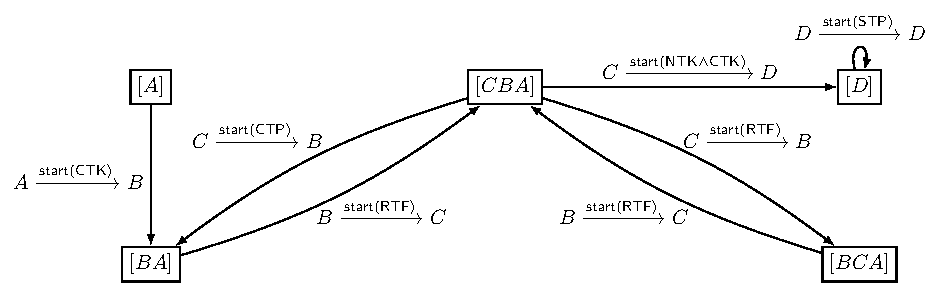
\includegraphics[scale = 0.75]{ifasm-example.pdf}
		\caption{Configurations reachable from the initial configuration $[A]$ in an $\IFAMASS$ $\Mm$}
		%in $\phi$
		% \vspace{-6mm}	
		\label{ifasm-example}
	\end{figure}
\end{example}
% In this case, we assume that the launch modes of activities are $\STD$.  Intuitively, for a transition $A\xrightarrow{\startactivity(\phi)}B$, the intent flags in $\phi$ may depend on each other. The dependency can exhibit in the following two forms: (1) $n$ \emph{subsumes} $n'$, i.e., $n'$ is ignored if $n$ co-occurs with $n'$, and the ``subsume'' relations are transitive, (2) $n$ \emph{enables} $n'$, i.e., $n'$ takes effect if $n$ co-occurs with $n'$. We summarize the dependencies among the intent flags in Figure xxx, 

% For a transition $A\xrightarrow{\startactivity(\phi)}B$, we conclude that :
% \begin{itemize}
	% 	\item when $\ctkflag$ tasks effect, then the task will be cleared, and $B$ is pushed into the task,
	% 	\item when $\ctpflag$ tasks effect, then the task will be poped until the top activity is $B$ when $B$ is in the task, $B$ will be pushed into the task otherwise, which is similar with the case $\lmd(B) = \STK$,
	% 	\item when $\rtfflag$ tasks effect, then $B$ is escalated to the top of the task when $B$ is in the task, $B$ will be pushed into the task otherwise, 
	% 	\item when $\stpflag$ tasks effect, then $B$ is pushed into the task when the top activity of the task is not $B$, which is similar with the case $\lmd(B) = \STP$.
	% \end{itemize}




\subsection{Configuration reachability of $\STK$-dominating $\IFAMASS$}
Let us assume that $\Mm = (\act, A_0, \lmd, \aft, \Delta)$ is an $\STK$-dominating $\IFAMASS$, that is, for all activities $A \in \act$, $\lmd(A) = \standard$ and $\aft(A) = \aft(A_0)$, moreover, for each transition $A \xrightarrow{\startactivity(\phi)} B \in \Delta$, we have $\phi \models \neg \ntkflag$. As a result, there is only one task in each configuration of $\Mm$.
Nevertheless, the reachability problem of $\Mm$ is far from trivial, since in a transition $A \xrightarrow{\startactivity(\phi)} B$ such that $\phi \models \neg \ctpflag \wedge \rtfflag$, if there is at least one occurrence of $B$ in the task, then $B$ will be moved to the top of the task. In other words, the $\rtfflag$ flag requires modifying not only the top symbol of the task, but also the non-top symbols. 

Our main idea to solve the reachability problem of $\STK$-dominating $\IFAMASS$ is to simulate the behavior of the $\rtfflag$ flag as a transduction on the contents of the task. As mentioned before, {\TrPDS} is a model that extends pushdown systems with transductions, where the closure of transductions is required to be finite. Nevertheless, as we shall see later on, the closure of transductions used to simulate $\rtfflag$ is infinite. To tackle this issue, we introduce a new decidable extension of pushdown systems with transductions, called pushdown system with well-partially-ordered transductions (\WOTrPDS), where the transduction closure can be infinite. 

In the sequel, we first define {\WOTrPDS} and prove the decidability of its reachability problem (Section~\ref{sec-wpotrpds}). Then we show how to utilize {\WOTrPDS} to solve the reachability problem of $\Mm$ (Section~\ref{sec-ifamass-reach}). 

%%%%%%%%%%%%%%%%%%%%%%%%
%%%%%%%%%%%%%%%%%%%%%%%%
\hide{
In this case, there is only one task in $\Mm$, then the configuration reachability problem of $\Mm$ is defined as follows: 
\begin{quote}
Given an $\NFA$ $\Aut$ over the alphabet $\act$, decide whether $\ConfSet(\Aut)\cap \RConfs(\Mm) \neq \emptyset$.
\end{quote}
Recall that the definition of $\STK$-dominating $\IFAMASS$, then we let $\tau= A\xrightarrow{\startactivity(\bot)}B$ and let $\rho = (S_1, \cdots, S_n)$ be the current configuration for some $n \ge 1$ and $\topact(\rho) = A$,  we define the semantics of $\STK$-dominating $\IFAMASS$ as follows:
\begin{itemize}
	\item If $\phi \models\ctpflag$ and $B \in \toptsk(\rho)$, then $\rho' =\clrtop(\rho, B)$,
	\item Otherwise,
	\begin{itemize}
		\item if $\phi \models \rtfflag$ and $B \in \toptsk(\rho)$, then $\rho'=\mvacttop(\rho, B)$,
		\item otherwise,
		\begin{itemize}
			\item if $\phi \models \stpflag$ and $B = \topact(\rho)$, then $\rho' = \rho$,
			\item otherwise, $\rho' = \push(\rho, B)$.
		\end{itemize}
	\end{itemize}
\end{itemize}
%
Our approach to tackle the configuration reachability problem of $\Mm$ is to simulate $\Mm$ by an extension of {\TrPDS}, i.e., pushdown systems with well-partially-ordered transductions ({\WOTrPDS}). In {\WOTrPDS}, the closure of transductions admits a basis which is well-partially-ordered with respect to the superset relation.
Theorem~\ref{thm-wstrpds-reach} shows the regular reachability problem of {\WOTrPDS} is decidable and Section~\ref{sec-proof-reach} proves the configuration reachability problem of $\STK$-dominating $\AMASS$ in this case is decidable.

Recall that there are four behaviors of $\Mm$ in this case, i.e., $\push$, $\mvacttop$, $\clrtop$ and $\Pop$.
The basic idea is to simulate the behaviorss of $\Mm$ by the transition rules of a {\TrPDS} $\Pp_{\Mm}$. While it is relatively easy to simulate the behaviors $\push, \clrtop, \Pop$, %by the transition rules of $\Pp_\Aut$, 
it is challenging to simulate $\mvacttop$. Given a transition $A\xrightarrow{\startactivity(\phi)}B$ with $\phi\models\rtfflag\wedge\neg\ctpflag$, the semantics requires to move the topmost occurrence of $B$ (if there is any) to the top of $\rho$. The most direct way to simulate it with $A \neq B$ is by two transition rules $p \xrightarrow{A / B | \tau_{B, A}} p$ and  $p \xrightarrow{A / BA | \tau_{\not B}} p$
%\jl{this should be $p \xrightarrow{A / BA | \tau_{\not B}} p$}
(where $p$ is a state in $\Pp_\Mm$), corresponding to the two situations that $B$ occurs/does no occur in the stack, where 
\begin{itemize}
\item $\tau_{B, A}$ is the transduction that removes the first occurrence of $B$ from the input string and adds $A$ in the beginning, and
%
\item $\tau_{\not B}$ checks that $B$ does not occur in the input string but keeps the input string unchanged. 
\end{itemize}
}
%%%%%%%%%%%%%%%%%%%%%%%%

\subsection{Pushdown system with well-partially-ordered transductions}\label{sec-wpotrpds}

\begin{definition}[Union-basis of transduction sets]\label{def-ubasis}
Let $\TranSet$ be a set of transductions and $\Tranbasis \subseteq \TranSet$. Then $\Tranbasis$ is called a \emph{union-basis} of $\TranSet$ if each $\tau \in \TranSet$ is equivalent to a finite union of transductions from $\Tranbasis$ (called a $\Tranbasis$-representation of $\tau$). 
%Moreover, if $\tau \in \TranSet$ is equivalent to $\tau_1 \cup \cdots \cup \tau_n$ with $\tau_i \in \Tranbasis$ for every $i \in [n]$, then $\tau_1 \cup \cdots \cup \tau_n$ is called a $\Tranbasis$-representation of $\tau$.
\end{definition}

%We are ready to define pushdown systems with well-partially-ordered transductions.
\begin{definition}[\WOTrPDS] \label{def:defatpds}
    A \emph{pushdown system with well-partially-ordered transductions} (\WOTrPDS) is a tuple $\Pp = (P, \Gamma, \TranSet, \Delta)$, 
    where $P$ is a finite set of $control\ states$, $\Gamma$ is a finite $stack\ alphabet$, $\TranSet \subseteq \UTrans$ is a finite set of letter-to-letter transductions, and $\Delta \subseteq P \times \Gamma \times \Gamma^{\le 2} \times \TranSet \times P$ is a finite set of transition rules, where $\Gamma^{\le 2} = \{\varepsilon\} \cup \Gamma \cup \Gamma \times \Gamma$. In other words, each transition in $\Delta$ is of one of the following forms, $(p, \gamma, \varepsilon, \tau, p')$, $(p, \gamma, \gamma',\tau, p')$, or $(p, \gamma, \gamma'_1 \gamma'_2, \tau, p')$ such that $\gamma, \gamma', \gamma'_1, \gamma'_2 \in \Gamma$ and $\tau \in \TranSet$. 
   Moreover, it is required that there is a union-basis $\Tranbasis \subseteq \langle \TranSet \rangle$ such that 
   \begin{itemize}
   \item $\{\emptyset, \tau_{\varepsilon}\} \subseteq \Tranbasis$,  (note here $\tau_{id}$ may not be in $\Tranbasis$)
   %
   \item  $(\Tranbasis, \preceq)$ is a wpo, namely, it satisfies DCC and does not contain infinite antichains, and
%
   \item for each $\tau \in \langle \TranSet \rangle$, a $\Tranbasis$-representation $\beta_\tau = \beta_{\tau, 1} \cup \cdots \cup \beta_{\tau, n_\tau}$ can be computed effectively, 
%
   \item $\preceq$ is union-distributive over $\Tranbasis$-representations, specifically, for each $\beta \in \Tranbasis$ and $\tau \in \langle \TranSet \rangle$ whose $\Tranbasis$-representation is $\beta_\tau=\beta_{\tau, 1} \cup \cdots \cup \beta_{\tau, n_\tau}$, if $\tau \preceq \beta$, then $ \beta_{\tau, i} \preceq \beta$ for some $i \in [n_\tau]$.
\end{itemize}
   % can be effectively rewritten as a finite union of transductions from $\Tranbasis$.
%   $(\langle \TranSet \rangle, \preceq)$ is a wpo, namely, it satisfies DCC and does not contain infinite antichains.
%The size of $\Pp$, denoted by $|\Pp|$, is defined as $|\Delta|$.
\end{definition}
For readability, we usually write a transition $(p, \gamma, w, \tau, p') \in \Delta$ as $p \xrightarrow{\gamma/w | \tau} p'$.

%Let $\Pp = (P, \Gamma, \TranSet, \Delta)$ be  a {\WOTrPDS}. 
A \emph{configuration} $c$ of $\Pp$ is a pair $(p, w)$, where $w = \gamma_1 \cdots \gamma_k \in \Gamma^*$ is the  stack content with $\gamma_1$ as the topmost symbol. We define a binary relation $\xrightarrow{\Pp}$ over the set of configurations as follows. Given two configurations $(p_1, w_1)$ and $(p_2, w_2)$, $(p_1, w_1) \xrightarrow{\Pp} (p_2, w_2)$ if $w_1 = \gamma w'_1$, and one of the following conditions holds,
\begin{itemize}
\item $p_1 \xrightarrow{\gamma/\varepsilon|\tau} p_2$ for some $\tau$ with  $w_2 \in \tau(w'_1)$, 
%
\item $p_1 \xrightarrow{\gamma/\gamma'|\tau} p_2$ for some $\gamma'$ and $\tau$ with $w_2 = \gamma' w'_2$ for some $w'_2 \in \tau(w'_1)$, 
%
\item $p_1 \xrightarrow{\gamma/\gamma' \gamma''|\tau} p_2$ for some $\gamma', \gamma''$ and $\tau$ with $w_2 = \gamma' \gamma'' w'_2$ for some $w'_2 \in \tau(w'_1)$.
\end{itemize}
Moreover, we use $\xRightarrow{\Pp}$ to denote the reflexive and transitive closure of $\xrightarrow{\Pp}$. We say that $(p_2, c_2)$ is \emph{reachable} from $(p_1, c_1)$ if $(p_1, c_1) \xRightarrow{\Pp} (p_2, c_2)$.
\begin{figure}[htb]
    \centering
	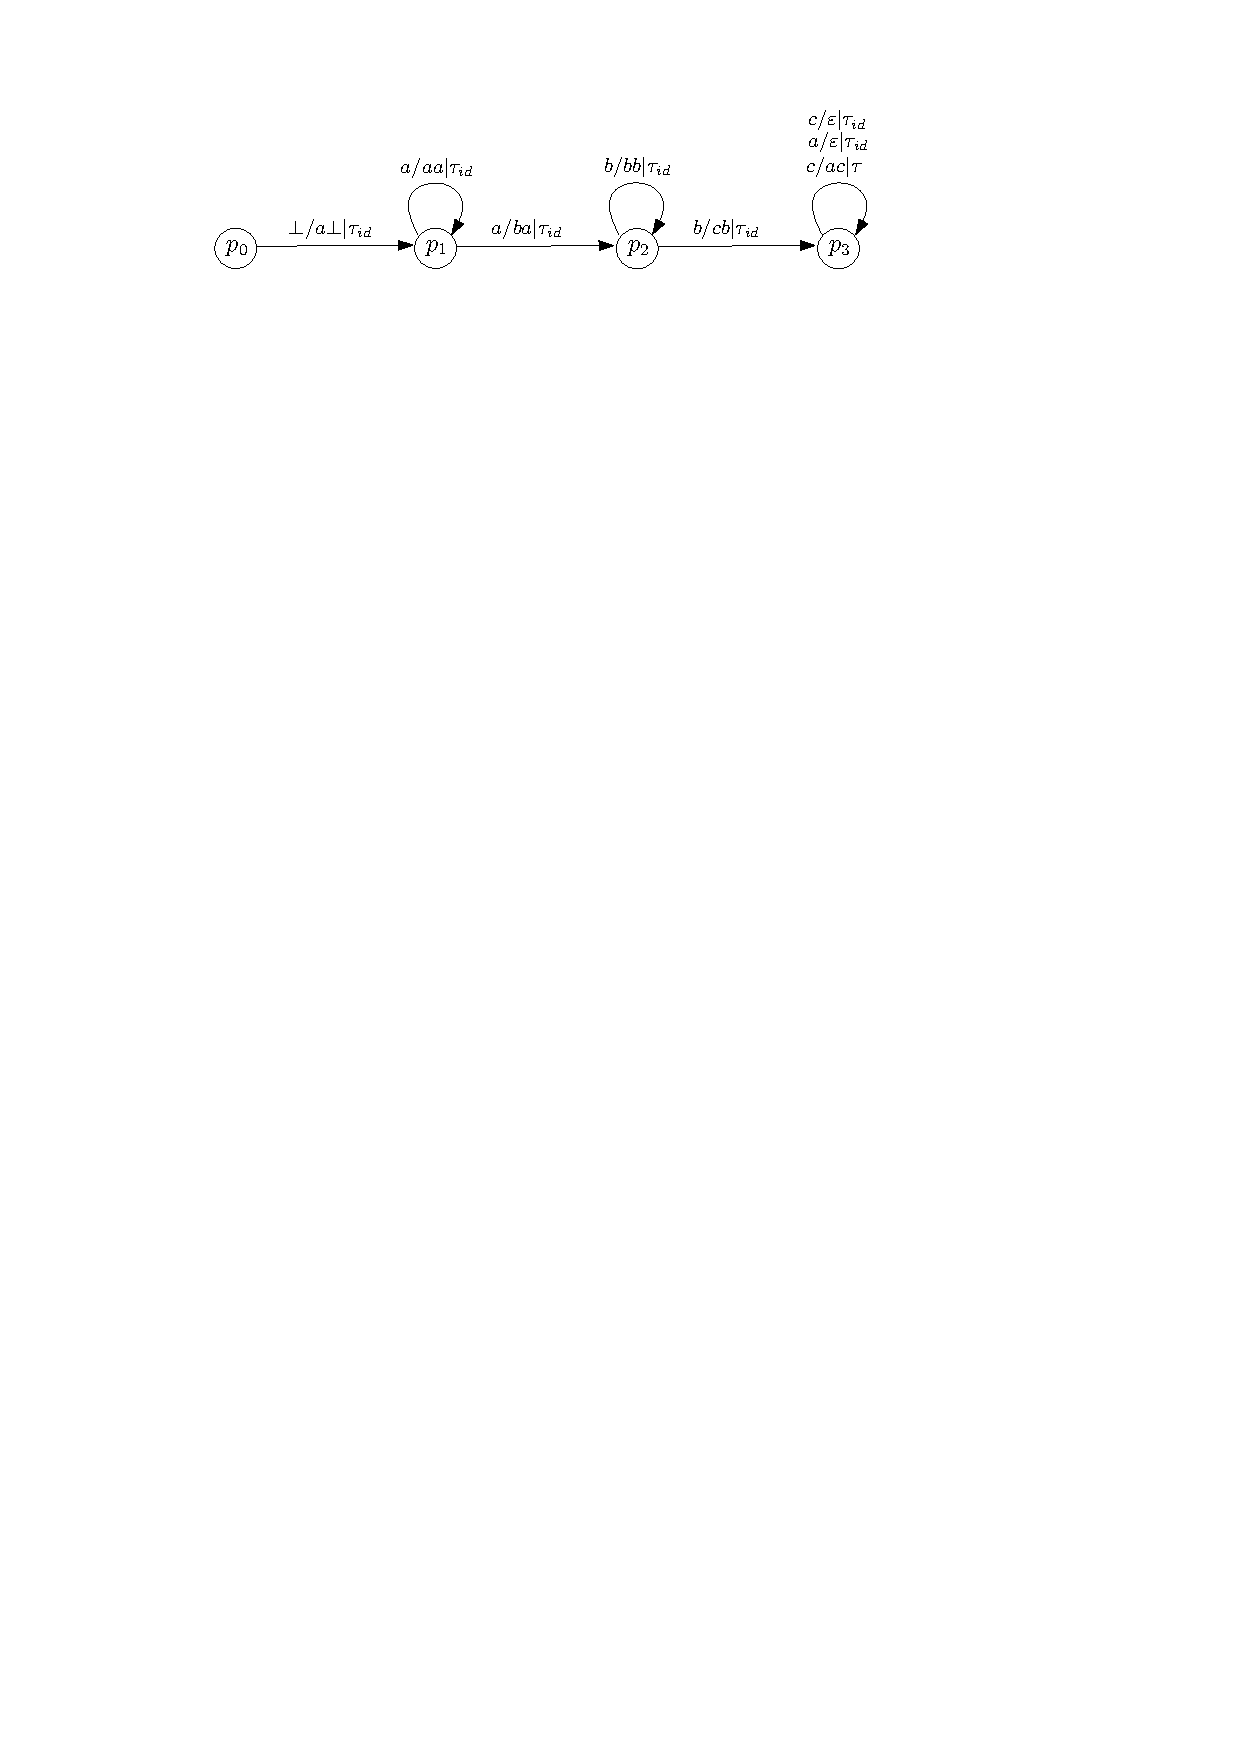
\includegraphics[scale = 0.9]{wstrpds-example.pdf}
	\caption{An example for \WOTrPDS}\label{fig-wstrpds-exmp}
\end{figure}

\begin{example}\label{exmp-wpotrpds}
Consider the {\WOTrPDS} $\Pp=(P, \Gamma, \TranSet, \Delta)$ (see Figure~\ref{fig-wstrpds-exmp}), where 
\begin{itemize}
\item $P = \{p_0, p_1, p_2, p_3\}$,  $\Gamma = \{\bot, a, b, c, d\}$,
% 
\item $\TranSet = \{\tau_{id}, \tau\}$, where $\tau$ is the transduction defined as follows: upon an input $w \in \Gamma^*$ where $a$ occurs at least once, it replaces at least the first occurrence of $a$ by $d$, more precisely, it nondeterministically chooses some $n \ge 1$ and replaces each of the first $n$ occurrences of $a$ in $w$ by $d$, for instance, $\tau(babad\bot) = \{bdbad\bot, bdbdd\bot\}$,
%
\item $\Delta$ is as illustrated in Figure~\ref{fig-wstrpds-exmp}, in particular, $(p_3, c, ac, \tau, p_3) \in \Delta$. 
%\left\{
%\begin{array}{l}
%(q_0, \bot, a\bot, \tau_{id}, q_1), (q_1, a, aa, \tau_{id}, q_1), (q_1, a, ba, \tau_{id}, q_2), (q_2, b, bb, \tau_{id}, q_2), \\
%(q_2, b, cb, \tau_{id}, q_3), (q_3, c, ac, \tau_1, q_3), (q_3, a, \epsilon, \tau_{id}, q_3) 
%\end{array}
%\right\}$.
\end{itemize}

From the definition of $\Delta$, $(p_3, bbdd\bot)$ is reachable from $(p_0, \bot)$, as witnessed by the following path in $\xrightarrow{\Pp}$, 
\[
\begin{array}{l}
(p_0, \bot) \xrightarrow{\Pp} (p_1, a \bot) \xrightarrow{\Pp} (p_1, aa \bot) \xrightarrow{\Pp} (p_2, baa \bot)  \xrightarrow{\Pp} (p_2, bbaa \bot)  \xrightarrow{\Pp} (p_3, cbbaa \bot)  \\
\xrightarrow{\Pp} (p_3, acbbdd \bot) \xrightarrow{\Pp} (p_3, cbbdd \bot)  \xrightarrow{\Pp} (p_3, bbdd \bot). 
\end{array}
\]
Note that, from the configuration $(p_3, cbbaa \bot)$, the transition $p_3 \xrightarrow{c/ac|\tau } p_3$ is applied. Then  $bbaa$ is transformed by $\tau$ into $bbdd$, moreover, $a$ is pushed. Therefore, the configuration $(p_3, acbbdd)$ is produced.

It is necessary to verify that $(\langle \TranSet \rangle, \preceq)$ has a well-partially-ordered union-basis $\Tranbasis$. First, we observe that $\tau^1 \supseteq \tau^2 \supseteq \cdots$, where $\tau^i$ for $i \ge 1$ is the $i$-fold composition of $\tau$, more specifically, $\tau^i$ nondeterministically replaces each of the first $n $ occurrences of $a$ in an input $w$ by $d$ for some $n \ge i$. It follows that $\tau^i \cup \tau^j = \tau^i$ for every $i < j$.
Moreover, $\lceil a, d \rfloor^{-1} \tau = \tau_{id} \cup \tau$. Therefore, the transduction closure $\langle \TranSet \rangle$ is $\{\emptyset, \tau_{id}, \tau_\varepsilon\} \cup \{\tau^i \mid i \ge 1\} \cup \{\tau_{\varepsilon} \cup \tau^i \mid i \ge 1\} \cup \{\tau_{id} \cup \tau^i \mid i \ge 1\}$. Let $\Tranbasis = \{\emptyset, \tau_{id}, \tau_\varepsilon\} \cup \{\tau^i \mid i \ge 1\}$. Then $\Tranbasis$ is a union-basis of $\langle \TranSet \rangle$. 
%, where $\tau^i$ is the $i$-fold composition of $\tau$, more specifically, $\tau^i$ nondeterministically replaces each of the first $n $ occurrences of $a$ in $w$ by $d$ for some $n \ge i$. 
%Note that $\tau_i$ is obtained as the $i$-fold composition of $\tau$. 
%
From $\tau^1 \supseteq \tau^2 \supseteq \cdots$, we deduce that each infinite descending chain of $(\Tranbasis, \preceq)$, i.e. each infinite ascending chain of $(\Tranbasis, \subseteq)$, eventually stabilizes at $\emptyset, \tau_{id}, \tau_\varepsilon$, or $\tau^i$ for some $i$. Thus $(\Tranbasis, \preceq)$ contains no infinite strictly descending chains, i.e. it satisfies the DCC condition. Moreover, from $\tau^1 \supseteq \tau^2 \supseteq \cdots$, we know that it contains no infinite antichains as well. We conclude that $(\Tranbasis, \preceq)$ is a wpo. The distributivity of $\preceq$ over $\Tranbasis$-representations is evident. \qed
%
%An example of {\WSTrPDS} here.
\end{example}

\begin{theorem}\label{thm-wstrpds-wpo}
	Given a {\WOTrPDS} $\Pp = (P, \Gamma, \TranSet, \Delta)$, and $\Tranbasis$ is the union-basis of $\langle \TranSet \rangle$, then $\overline{\Tranbasis}$ is the union-basis of $\langle \overline{\TranSet}\rangle$.
\end{theorem}
We prove Theorem~\ref{thm-wstrpds-wpo} by showing $\overline{\Tranbasis}$ satisfied the four conditions in Definition~\ref{def:defatpds}.
\begin{proof}
	First, by the definition of $\overline{\Tranbasis}$, we have that $\{\emptyset, \tau_{\epsilon}\}\subseteq \overline{\Tranbasis}$.

	Now we prove $(\overline{\Tranbasis}, \preceq)$ is a wpo. By the definition of $\overline{\Tranbasis}$, for every $\overline{\beta_1},\overline{\beta_2}\in\overline{\Tranbasis}$, if $\overline{\beta_1}\neq\emptyset$ and $\overline{\beta_2}\neq \emptyset$, then $\overline{\beta_1}\preceq\overline{\beta_2}$ iff $\beta_1\preceq\beta_2$. Since $(\Tranbasis, \preceq)$ is a wpo, we deduce that $(\overline{\Tranbasis}, \preceq)$ is a wpo.

	Then we prove for each $\overline{\tau}\in\langle\overline{\TranSet}\rangle$, a $\overline{\Tranbasis}$-representation $\beta_{\overline{\tau}}$ can be computed effectively.
	Since $\langle\overline{\TranSet}\rangle = \overline{\langle \TranSet \rangle}$, then for each $\overline{\tau}\in\langle\overline{\TranSet}\rangle$, we have $\tau \in \langle \TranSet \rangle$. 
	Suppose that $\tau$ can be rewritten into the $\Tranbasis$-representation $\beta_1\cup\cdots\cup\beta_m$, then it is easy to observe that $\overline{\tau} = \overline{\beta_1}\cup\cdots\cup\overline{\beta_m}$, where $\overline{\beta_1},\cdots,\overline{\beta_m} \in \overline{\Tranbasis}$. Therefore $\overline{\beta_1}\cup\cdots\cup\overline{\beta_m}$ is the $\overline{\Tranbasis}$-representation of $\overline{\tau}$.

	Finally, we prove $\preceq$ is union-distributive over $\overline{\Tranbasis}$-representations, specifically, for each $\overline{\beta} \in \overline{\Tranbasis}$ and $\overline{\tau} \in \langle \overline{\TranSet} \rangle$ whose $\overline{\Tranbasis}$-representation is $\beta_{\overline{\tau}}=\beta_{\overline{\tau}, 1} \cup \cdots \cup \beta_{\overline{\tau}, n_{\overline{\tau}}}$, if $\overline{\tau} \preceq \overline{\beta}$, then $ \beta_{\overline{\tau}, i} \preceq \overline{\beta}$ for some $i \in [n_{\overline{\tau}}]$.

	For each $\overline{\beta} \in \overline{\Tranbasis}$ and $\overline{\tau} \in \langle \overline{\TranSet} \rangle$ whose $\overline{\Tranbasis}$-representation is $\beta_{\overline{\tau}}=\beta_{\overline{\tau}, 1} \cup \cdots \cup \beta_{\overline{\tau}, n_{\overline{\tau}}}$, we have that $\beta\in\Tranbasis$ and $\tau = \beta_{\tau,1}\cup \cdots \cup \beta_{\tau,n_\tau} \in \TranSet$, where $n_\tau = n_{\overline{\tau}}$ and for each $i\in[n_\tau]$, $\beta_{\overline{\tau}, i} = \overline{\beta_{\tau, i}}$.
	Then if $\overline{\tau}\preceq\overline{\beta}$, we have $\tau \preceq \beta$, i.e., $\beta\subseteq \tau$. Since $\Tranbasis$ is the union-basis of $\langle \TranSet \rangle$, we have $\beta_{\tau, i}\preceq \beta$, i.e., $\beta\subseteq\beta_{\tau, i}$ for some $i\in[n_\tau]$. Then we have $\overline{\beta}\subseteq \beta_{\overline{\tau}, i}$, i.e., $\beta_{\overline{\tau}, i} \preceq \overline{\beta}$.
	\qed

\end{proof}

In this paper, we consider the \emph{regular reachability problem} of {\WOTrPDS}.
\begin{quote} 
	Given a {\WOTrPDS} $\Pp = (P, \Gamma, \TranSet, \Delta)$, control states $p_1, p_2 \in P$, regular languages $L_1, L_2$ over $\Gamma$, determine whether there exist %strings $w_1, w_2$ such that 
	$w_1 \in L_1$, $w_2 \in L_2$ such that $(p_1, w_1) \xRightarrow{\Pp} (p_2, w_2)$.
\end{quote}
%\begin{itemize}
%\item The \emph{reachability problem} is to check for two given configurations $(q_1, w_1)$ and $(q_2, w_2)$, whether $(q_1, w_1) \xRightarrow{\Pp} (q_2, w_2)$.
%
%\item 
%\end{itemize}

%We will show that the regular reachability problem of {\WOTrPDS} is decidable. In the next section, a model called finite automata with well-ordered transductions will be introduced, to represent sets of configurations of {\WOTrPDS}.


\begin{theorem}\label{thm-wstrpds-reach}
The regular reachability problem of {\WOTrPDS} is decidable.
\end{theorem}

Fix a  {\WOTrPDS} $\Pp = (P, \Gamma, \TranSet, \Delta)$. %and $\Aut = (Q, \Gamma, \delta, P, F)$ be a $\Pp$-{\NFA}. 
We show Theorem~\ref{thm-wstrpds-reach} via the saturation technique, which %by applying the saturation procedures from \cite{SM+15,Song18}. 
requires to represent the set of reachable configurations of $\Pp$. For traditional pushdown systems, a tailored {\NFA} (commonly referred to as P-automata in literature) suffices. For {\WOTrPDS}, we %generalize P-automata to 
introduce a new model, viz., \emph{finite automata with well-partially-ordered transductions} ({\WOTrNFA}), in Section~\ref{sec-wotrnfa}. 
Then in Section~\ref{sect:decidability}, we utilize the saturation technique to reduce the regular reachability problem of {\WOTrPDS} %the decidability % by reducing 
to the intersection problem of {\WOTrNFA} and {\NFA}, which is shown to be decidable in Section~\ref{sec:fatrnfa}.

%We prove Theorem~\ref{thm:st-amass-reach} by showing that a {\WOTrPDS} $\Pp_\Mm = (P_\Mm, \Gamma_\Mm, \TranSet_\Mm, \Delta_\Mm)$ can be constructed from a given {\AMASS} $\Mm = (\act, A_0,\lmd,\aft,\Delta)$ to simulate the behaviors of $\Mm$. We show the details in Section~\ref{sec-proof-reach}


\subsubsection{Finite automata with well-partially-ordered transductions}\label{sec-wotrnfa}
 
\begin{definition}[{\WOTrNFA}] %[Finite automata with finite ascending chians and antichains transductions]
	Given a {\WOTrPDS} $\Pp=(P, \Gamma, \TranSet, \Delta)$ with $\Tranbasis$ as the union-basis of $\langle \TranSet \rangle$, a $\Pp$-{\WOTrNFA} is a tuple $\Aut =(Q, \Gamma, \delta, I, F)$,
	where $Q$ is the set of states such that $P \subseteq Q$, $I\subseteq P\subseteq Q$ is the set of initial states, $F \subseteq Q$ is the set of final states,  
	%and the set of initial states is $P$, %is a finite set of states, $\Sigma$ is a finite alphabet, 
	%$\TranSet$ is a finite set of transductions, %$I \subseteq Q$ (reps. $F \subseteq Q$) is a finite set of initial (reps. final) states, 
	and $\delta \subseteq Q \times \Gamma_\varepsilon \times \Tranbasis \times Q$ is a finite set of transition rules.

    A $\Pp$-{\WOTrNFA} $\Aut$ is called a {$\Pp$-{\NFA}} if for every $(q, a, \beta, q')$, $\beta = \tau_{id}$. 
\end{definition}

For convenience, we write a transition $(q, a, \beta, q')$ as $q \xrightarrow{a | \beta} q'$. 
To define the semantics of $\Aut$, we extend the transition rules $q \xrightarrow{a | \beta} q' \in \delta$  to a relation $q \xRightarrow{w | \tau} q'$ for a string $w$,  
%
%The relation $q \xRightarrow{w | \tau} q'$ is  
defined inductively as follows:
\begin{itemize}
	\item if $q \xrightarrow{a |\beta} q'$, then $q \xRightarrow{a | \beta} q'$, 
	%
	\item if $q \xRightarrow{w | \tau} q'$ and $q' \xrightarrow{b |\beta } q'' $, then $q \xRightarrow{w a | (\lceil a, b\rfloor^{-1}\tau) \circ \beta} q''$ for every $a \in \Gamma_\varepsilon$ such that $\lceil a, b\rfloor^{-1}\tau \neq \emptyset$.
\end{itemize}
Intuitively, $q \xRightarrow{w | \tau} q'$ means that in $\Aut$,  $q'$ is reached starting from $q$ after reading $w$. Moreover, the transduction $\tau$, which is  to be applied to the remaining suffix of the input string, is produced. Note that the transduction  $\tau \in \langle \TranSet \rangle$ in $q \xRightarrow{w | \tau} q'$ may not be in $\Tranbasis$. 

A configuration $(p, w)$ of $\Pp$ is accepted by $\Aut$ if $p\in I$ and $p \xRightarrow{w | \tau} q$ for some $q \in F$ and $\tau \in \langle \TranSet \rangle$ such that $(\varepsilon, \varepsilon) \in \tau$.
%
Let us use $\confs(\Aut)$ to denote the set of configurations of $\Pp$ accepted by $\Aut$.
Moreover, let $\Lang(\Aut)$ to denote the set of words $w$ such that $(p, w)\in\confs(\Aut)$ for some $p \in I$.
For a $\Pp$-$\WOTrNFA$ $\Aut = (Q, \Gamma, \delta, I, F)$, we use $\Aut(p')$ to denote to denote the $\Pp$-$\WOTrNFA$ obtained from $\Aut$ by replacing $I$ with $\{p'\}$.

It turns out that $\Pp$-{\WOTrNFA} is capable of representing \emph{non-regular} set of configurations, as %witnessed 
shown by the following example.
\begin{example}
Let $\Pp$ be the {\WOTrPDS} in Example~\ref{exmp-wpotrpds}. Consider the $\Pp$-{\WOTrNFA} $\Aut = (Q, \Gamma, \delta, I, F)$ in Figure~\ref{fig-ptrnfa-exmp}, where $F= \{q_1\}$ and $\tau$ is the transduction from $\Pp$ that replaces at least the first occurrence of $a$ by $d$. From $p_3 \xrightarrow{c | \tau} p_3$, $p_3 \xrightarrow{b | \tau_{id}} q_1$, we have $p_3  \xRightarrow{c b | (\lceil b, b\rfloor^{-1} \tau) \circ \tau_{id}} q_1$, thus $p_3 \xRightarrow{cb | \tau} q_1$. Moreover, from $q_1 \xrightarrow{d | \tau_{id}} q_1$, we deduce $p_3 \xRightarrow{c b a | (\lceil a, d\rfloor^{-1} \tau) \circ \tau_{id}} q_1$. Since $(\lceil a, d\rfloor^{-1} \tau) \circ \tau_{id} = \tau_{id} \cup \tau$, we have $p_3 \xRightarrow{c b a |  \tau_{id} \cup \tau} q_1$ and $(\epsilon, \epsilon) \in \tau_{id} \cup \tau$. Thus $(p_3, cba)$ is accepted by $\Aut$. On the other hand, although $p_3 \xRightarrow{cb | \tau} q_1$ with $q_1 \in F$, but $(\epsilon, \epsilon) \not \in \tau$, thus $(p_3, cb)$ is not accepted by $\Aut$.  Furthermore, we observe that for $m \ge 1$, $p_3 \xRightarrow{c^m | \tau^m} p_3$. From the fact that $\tau^m$ replaces at least $m$ occurrences of $a$ by $d$, we deduce that for each configuration of the form $(p_3, c^m b a^n)$ with $m,n \ge 1$, it is accepted by $\Aut$ iff $n \ge m$.  Therefore, $\confs(\Aut)$, the set of configurations accepted by $\Aut$, is non-regular. 
%
\begin{figure}[htb]
    \centering
	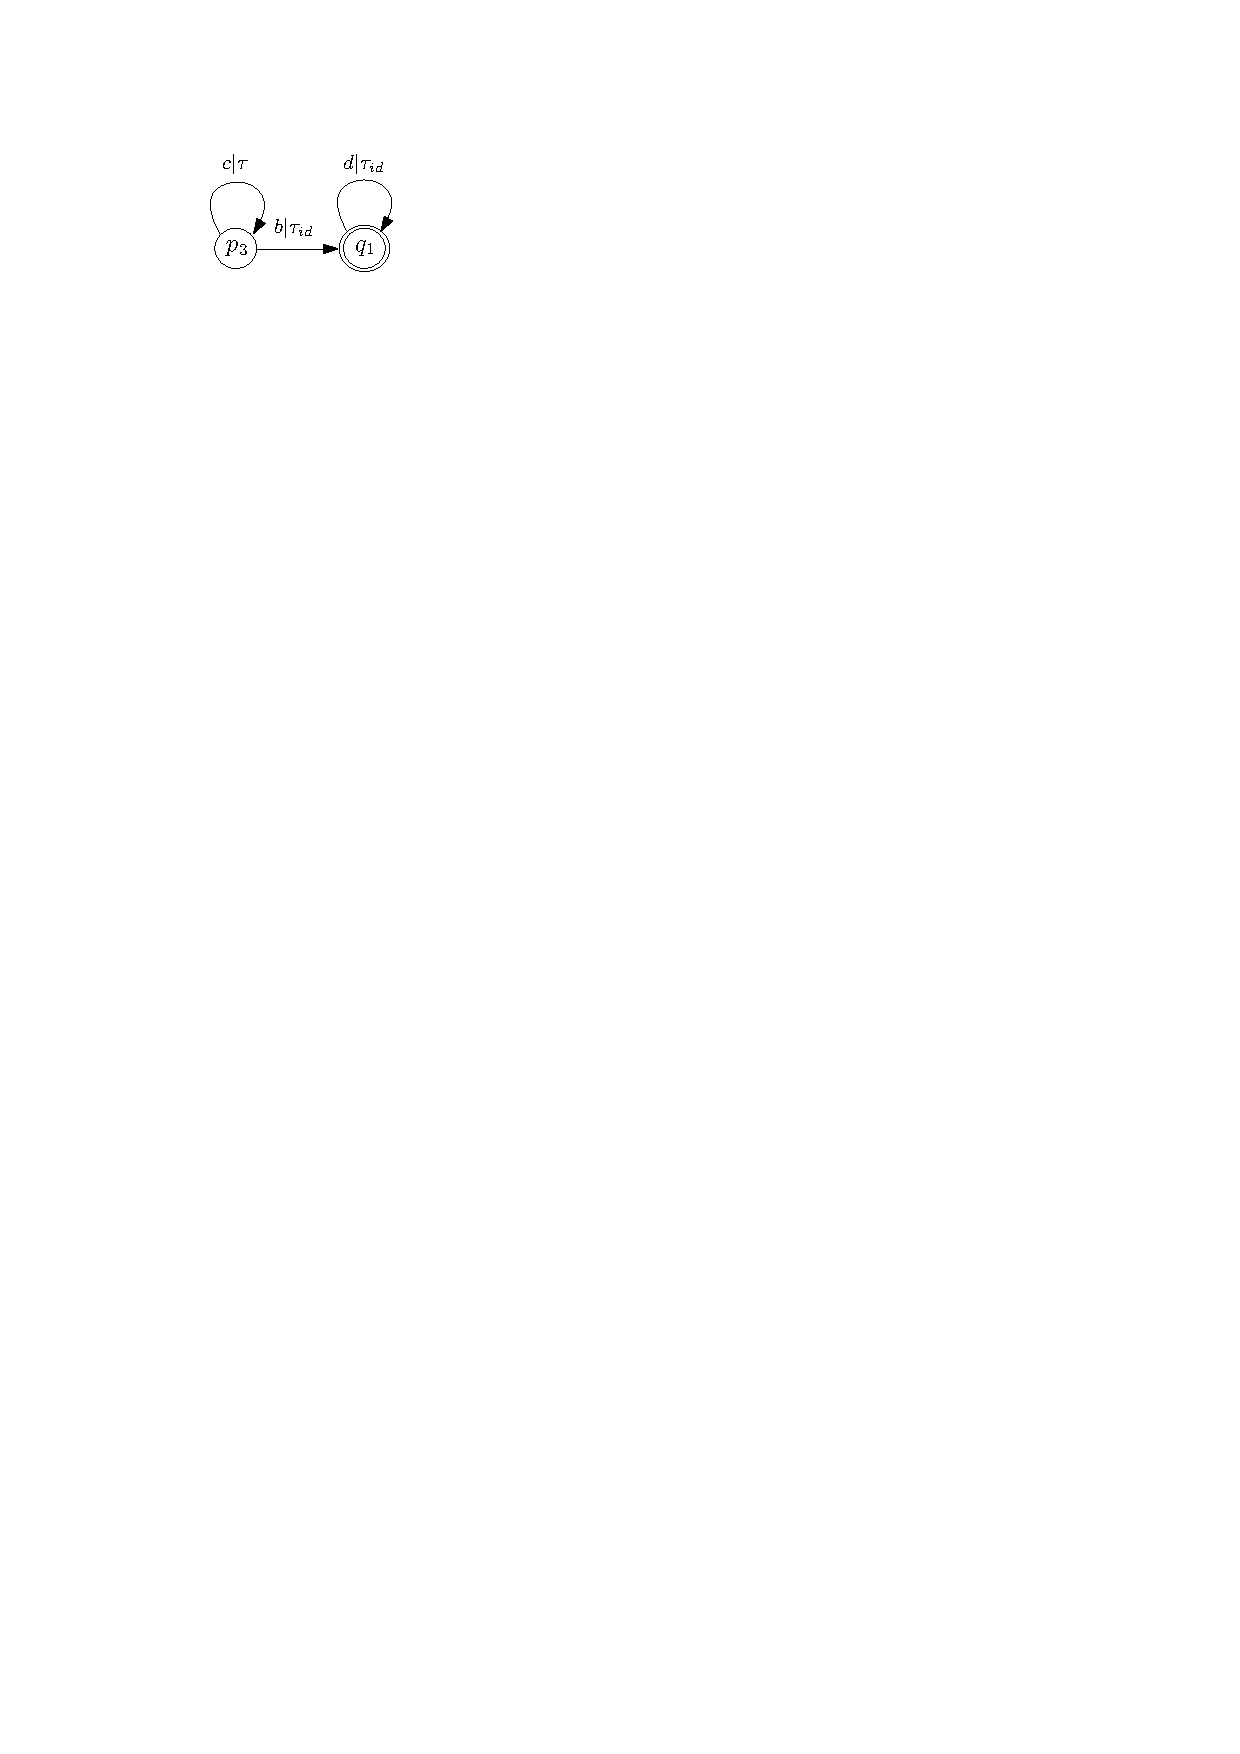
\includegraphics[scale = 0.9]{pwpotrnfa-example.pdf}
	\caption{An example of $\Pp$-\WOTrNFA}\label{fig-ptrnfa-exmp}
\end{figure}
\qed
\end{example}

For a $\Pp$-{\WOTrNFA} $\Aut$, $\pre^*_\Pp(\confs(\Aut))$  denotes the set of configurations $(p, w)$ of $\Pp$ such that $(p, w) \xRightarrow{\Pp} (p', w')$ for some $(p', w') \in \confs(\Aut)$. Accordingly, $\post^*_\Pp(\confs(\Aut))$ denotes the set of configurations $(p, w)$ of $\Pp$ such that $(p', w') \xRightarrow{\Pp} (p, w)$ for some $(p', w') \in \confs(\Aut)$.





%%%%%%%%%%%%%%%%%%%%%%%%%%%%%%%%%%%%%%%%%%%%%%%%%
%%%%%%%%%%%%%%%%%%%%%%%%%%%%%%%%%%%%%%%%%%%%%%%%%
\subsubsection{Saturation} \label{sect:decidability}
Let $\Pp = (P, \Gamma, \TranSet, \Delta)$ be a  {\WOTrPDS} where $\Tranbasis$, the union-basis of  $\langle \TranSet \rangle$, is a wpo, and let $\Aut = (Q, \Gamma, \delta, I, F)$ be a $\Pp$-{\WOTrNFA}. %We prove Theorem~\ref{thm-wstrpds-reach} by 
We apply the saturation procedures from \cite{SM+15,Song18} to obtain a $\Pp$-{\WOTrNFA} $\Aut^{\pre^*}_{\Pp}$ (resp. $\Pp$-{\WOTrNFA} $\Aut^{\post^*}_{\Pp}$), which represents $\pre^*_\Pp(\confs(\Aut))$ (resp. $\post^*_\Pp(\confs(\Aut))$).

% Let $\Pp = (P, \Gamma, \TranSet, \Delta)$ be a  {\WOTrPDS} where $\Tranbasis$, the union-basis of  $\langle \TranSet \rangle$, is a wpo, and let $\Aut = (Q, \Gamma, \delta, F)$ be a $\Pp$-{\NFA}. %We prove Theorem~\ref{thm-wstrpds-reach} by 
% We apply the saturation procedures from \cite{SM+15,Song18} to obtain a $\Pp$-{\WOTrNFA} $\Aut^{pre^*}$, which represents $pre^*_\Pp(\ConfSet(\Aut))$ and 
%represents the set of configurations reachable from the initial configuration. 
%The termination of the saturation procedures is guaranteed by the assumption that the transduction closure is well-ordered.  Then the regular reachability problem is reduced to the {\WOTrNFA}-{\NFA} intersection problem for $\Aut$ and $\AutB$, which is decidable according to Proposition~\ref{prop-wstrnfa-nfa-intersect}.
%
%In the sequel, we first recall the two saturation procedure in \cite{SM+15,Song18}, then prove its termination.
%
%Let $\Aut = (Q', \Gamma, \delta', P, F')$ be a $\Pp$-{\WOTrNFA} such that for each pair of states $(q_1, q_2)$ and each $\gamma \in \Gamma_\varepsilon$, there is at most one $\tau'' \in \langle \TranSet \rangle$ satisying that $(q_1, \gamma, \tau'', q_2) \in \delta'$. 
%
%The $\Pp$-{\WOTrNFA} $\Aut^{pre^*}$ 
\paragraph{Computing $\pre^*$}
$\Aut^{\pre^*}_{\Pp}$ is constructed by iteratively adding the transitions to $\Aut$, according to the following saturation rule. 
%$\Aa^{pre^*} $ is obtained from $\Aa$ by adding the transitions according to the following three saturation rules.

\smallskip

\fbox{
%
\begin{minipage}{0.9\textwidth}
%\begin{enumerate}
    Let $\Aut'$ be the current $\Pp$-{\WOTrNFA}.
     For $(p_1, \gamma, w, \tau, p_2) \in \Delta$ and $p_2  \xRightarrow{w\mid\tau'} q'$ in $\Aut'$, suppose that a $\Tranbasis$-representation of $\tau\circ\tau'$ is $\beta_1 \cup \cdots \cup \beta_n$ where $\beta_i \in \Tranbasis$ for each $i \in [n]$,  %we do the following: 
%     Suppose that a $\Tranbasis$-representation of $\tau\circ\tau'$ is $\beta_1 \cup \cdots \cup \beta_n$ where $\beta_i \in \Tranbasis$ for each $i \in [n]$.
     %
     for each $i \in [n]$ such that there does \emph{not} exist a transition $(p_1, \gamma, \tau'', q')$ in $\Aut'$ with $\tau'' \preceq \beta_i$ (i.e. $\tau'' \supseteq \beta_i$),  we update $\Aut'$ by adding a transition $(p_1, \gamma, \beta_i, q')$.
     %
%     if there is a transition $(p_1, \gamma, \tau'', q')$ in the current $\Pp$-{\WOTrNFA}, then we replace $(p_1, \gamma, \tau'', q')$ with the transition $(p_1, \gamma, (\tau\circ\tau') \cup \tau'', q')$, otherwise, we add a transition $(p_1, \gamma,\tau\circ\tau', q')$.
%\end{enumerate}
\end{minipage}
}
\smallskip

\paragraph{Computing $\post^*$}
$\Aut^{\post^*}_{\Pp}$ is constructed by iteratively adding the transitions to $\Aut$, according to the following saturation rule. 
%$\Aa^{pre^*} $ is obtained from $\Aa$ by adding the transitions according to the following three saturation rules.

\smallskip

\fbox{

\begin{minipage}{0.9\textwidth}
    Let $\Aut'$ be the current $\Pp$-{\WOTrNFA}. For $(p_1, \gamma, w, \tau, p_2) \in \Delta$, and $p_1  \xRightarrow{\gamma\mid\tau'} q'$ in $\Aut'$, 
    suppose that a $\Tranbasis$-representation of $\overline{\tau}\circ\tau'$ is $\beta_1 \cup \cdots \cup \beta_n$ where $\beta_i \in \Tranbasis$ for each $i \in [n]$, 
    \begin{enumerate}
        \item if $w = \epsilon$ or $w=\gamma_1$, for each $i \in [n]$ such that there does \emph{not} exist a transition $(p_2, w, \tau'', q')$ in $\Aut'$ with $\tau'' \preceq \beta_i$ (i.e. $\tau'' \supseteq \beta_i$),  we update $\Aut'$ by adding a transition $(p_2, w, \beta_i, q')$.
        \item if $w = \gamma_1\gamma_2$, 
            \begin{itemize}
                \item suppose that a $\Tranbasis$-representation of $\tau_{\id}$ is $\beta_1' \cup \cdots \cup \beta_m'$ where $\beta_i' \in \Tranbasis$ for each $i \in [m]$, then for each $i\in[m]$, we update $\Aut'$ by adding a transition $(p_2,\gamma_1,\beta_i',\langle p_2,\gamma_1\rangle)$,
                \item for each $i \in [n]$ such that there does \emph{not} exist a transition $(\langle p_2,\gamma_1\rangle, \gamma_2, \tau'', q')$ in $\Aut'$ with $\tau'' \preceq \beta_i$ (i.e. $\tau'' \supseteq \beta_i$), we update $\Aut'$ by adding a transition $(\langle p_2,\gamma_1\rangle, \gamma_2, \beta_i, q')$.
            \end{itemize}

    \end{enumerate}
\end{minipage}
}
\smallskip
%Note that the aforementioned saturation rule guarantees the following property is preserved in the construction: For each pair of states $(q_1, q_2)$ and each $\gamma \in \Gamma_\varepsilon$, there is at most one $\tau'' \in \langle \TranSet \rangle$ satisying that $(q_1, \gamma, \tau'', q_2) \in \delta'$.


We now show that the saturation procedure for computing $\Aut^{\pre^*}_{\Pp}$ terminates. 
%The proof for computing $\Aut^{pre^*}$ is similar.
%
Towards contradiction, suppose that 
%the saturation procedure for computing $\Aut^{pre^*}$ 
it does not terminate. From the construction of $\Aut^{\pre^*}_{\Pp}$, there must be $q_1, q_2 \in Q'$, $\gamma \in \Gamma_\varepsilon$, and an infinite sequence of transductions $\beta_1, \beta_2, \cdots \in \Tranbasis$ such that the transitions $(q_1, \gamma, \beta_1, q_2) $, $(q_1, \gamma, \beta_2, q_2) $, $\cdots$ are added one by one,  and for every $i > 1$ and $j \le i$, $\beta_j \not \preceq \beta_i$,  that is, either $\beta_j$ and $\beta_i$ are incomparable or $\beta_j \succ \beta_i$. From infinite Ramsey theorem (cf. Theorem 9.1.2 in \cite{Rein00}), there must be an infinite sequence $i_1 < i_2 < \cdots$ such that $\beta_{i_1}, \beta_{i_2}, \cdots$ is either an infinite antichain or an infinite strictly descending chain. This contradicts the assumption that $(\Tranbasis, \preceq)$ is a wpo. 
The proof for computing $\Aut^{\post^*}_{\Pp}$ is similar.
%$\tau_1 \subset \tau_2 \subset \cdots$, that is, $\tau_1, \tau_2, \cdots$ is a strictly ascending chain with respect to $\subseteq$, thus a strictly descending chain with respect to $\preceq$. This contradicts the assumption that $(\langle \TranSet\rangle, \preceq) $ is a wpo.


\begin{example}
Let us continue Example~\ref{exmp-wpotrpds}. Let $\Aut = (Q, \Gamma, \delta, I, F)$ be the $\Pp$-{\WOTrNFA} recognizing the configurations $\{(p_3, b^m d^n \bot) \mid m > 0, n > 0\}$ (see Figure~\ref{fig-pnfa-exmp}). More specifically, $Q= P \cup \{q_1, q_2, q_3\}$, $I = \{p_3\}$, $F= \{q_3\}$, and $\delta$ is illustrated by the edges in Figure~\ref{fig-pnfa-exmp} (where the identity transduction $\tau_{id}$ in the transitions is omitted).  
%More specifically, $Q = \{p_3, q_1, q_2\}$
%
\begin{figure}[htb]
    \centering
	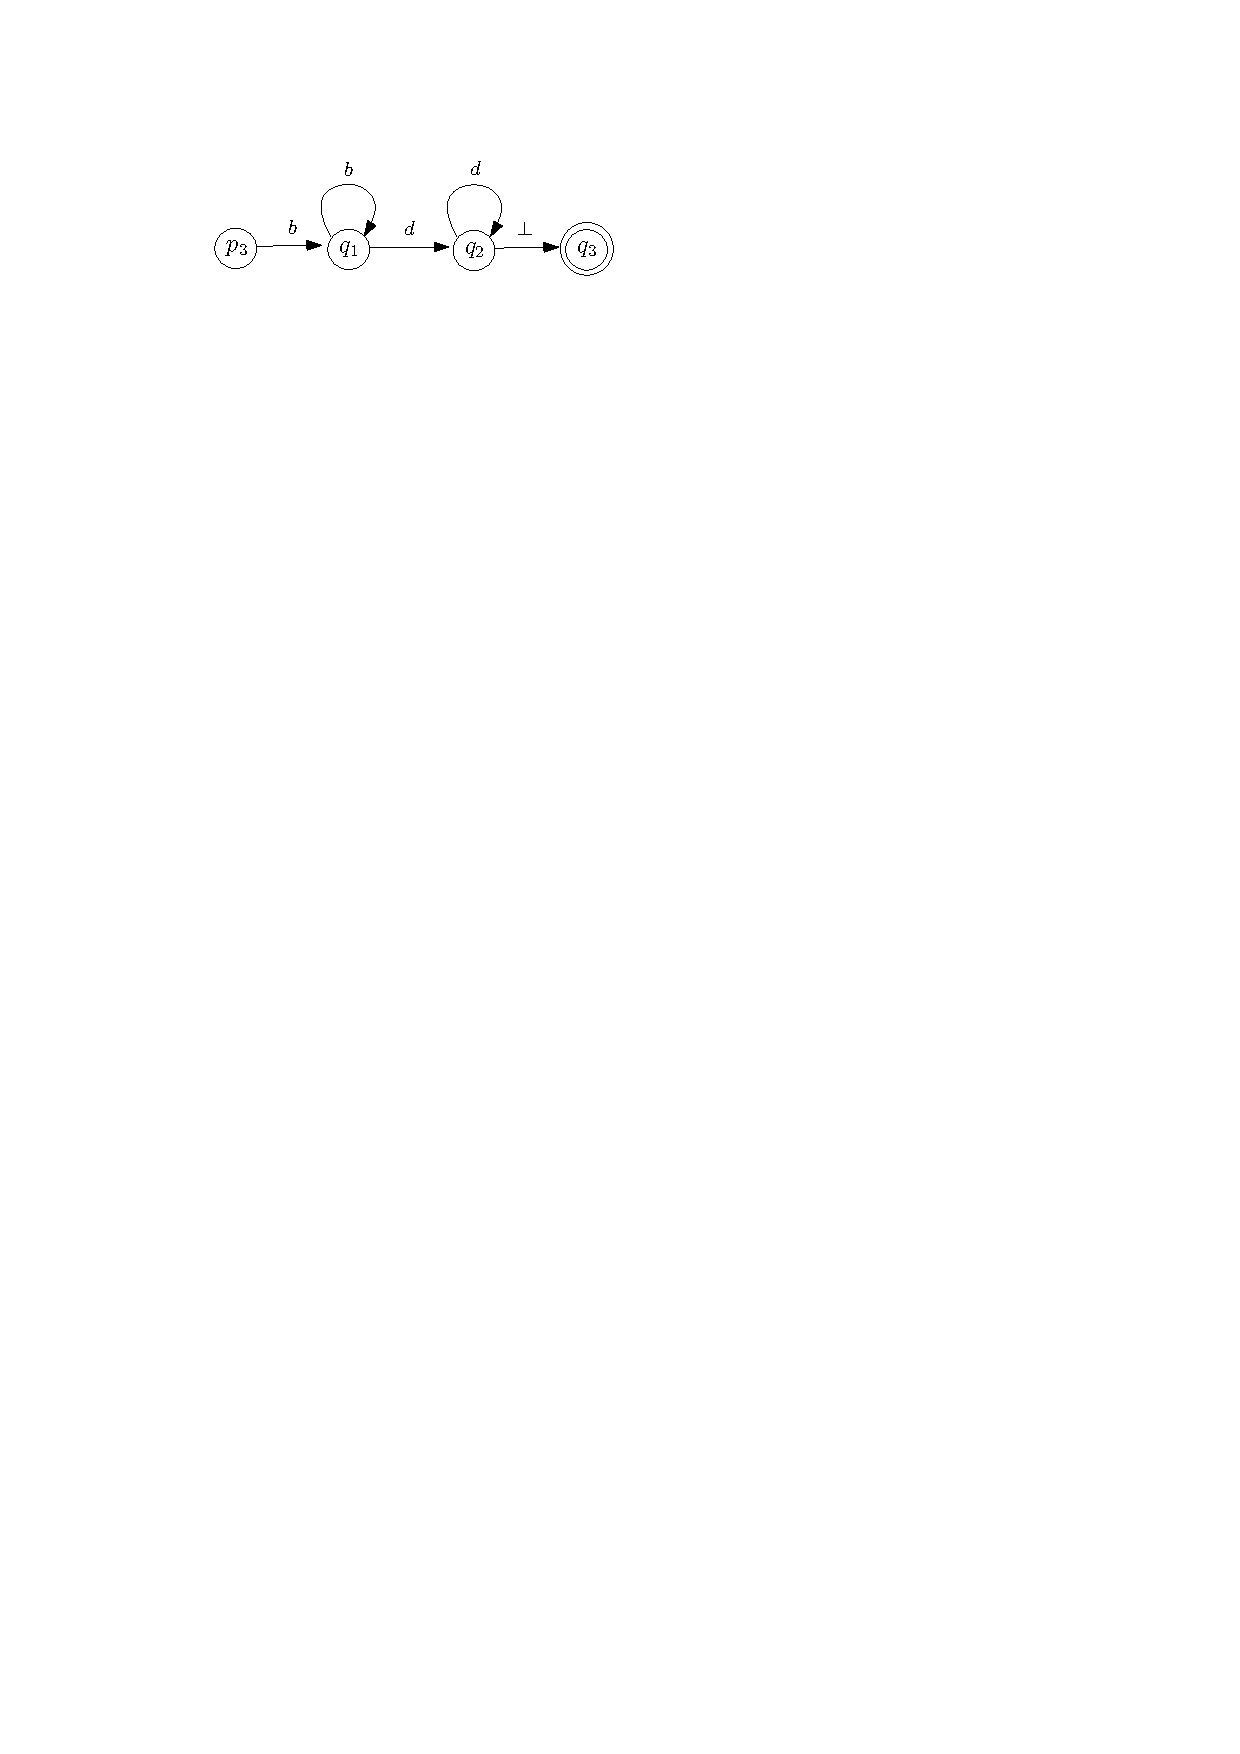
\includegraphics[scale = 0.9]{pnfa-example.pdf}
	\caption{An example of $\Pp$-{\WOTrNFA} $\Aut$}\label{fig-pnfa-exmp}
\end{figure}

Then we apply the saturation rule to add transitions.
\begin{itemize}
\item In the beginning, because $(p_3, a, \varepsilon, \tau_{id}, p_3) \in \Delta$ and $p_3 \xRightarrow{\varepsilon | \tau_{id}} p_3$ in $\Aut$, the transition $(p_3, a, \tau_{id}, p_3)$ is added according to the saturation rule. Similarly, the transition $(p_3, c, \tau_{id}, p_3)$ is added. 
%
\item Because $(p_3, c, ac, \tau, p_3) \in \Delta$, $p_3 \xRightarrow{ac | \tau_{id}} p_3$  in the current $\Pp$-{\WOTrNFA}, $\tau \circ \tau_{id} = \tau \in \Tranbasis$, and 
 there already exists a transition $(p_3, c, \tau_{id}, p_3)$, moreover, $\tau_{id} \not \preceq \tau$, the transition $(p_3, c, \tau, p_3)$ is added according to the saturation rule. 
%
\item Similarly, since $(p_2, b, cb, \tau_{id}, p_3) \in \Delta$, $p_3 \xRightarrow{cb | \tau_{id}} q_1$ and $p_3 \xRightarrow{cb | \tau} q_1$ in the current $\Pp$-{\WOTrNFA}, two transitions $(p_2, b, \tau_{id}, q_1)$  and $(p_2, b, \tau, q_1)$ are added. 
%
\item Furthermore, because $(p_1, a, ba, \tau_{id}, p_2) \in \Delta$ and $p_2 \xRightarrow{ba | \tau_{id} \cup \tau} q_2$ in the current $\Pp$-{\WOTrNFA} (This follows from $p_2 \xrightarrow{b | \tau} q_1$, $q_1 \xrightarrow{d | \tau_{id}} q_2$, and $(\lceil a, d\rfloor^{-1} \tau) \circ \tau_{id} = \tau_{id} \cup \tau$.), two transitions $(p_1, a, \tau_{id}, q_2)$  and $(p_1, a, \tau, q_2)$ are added.
%
%\item Furthermore, because $(p_2, b, cb, \tau_{id}, p_3) \in \Delta$, $p_3 \xRightarrow{cb | \tau} q_1$ in the current $\Pp$-{\WOTrNFA}, $ \tau_{id} \circ \tau = \tau \in \Tranbasis$, and there already exists a transition $(p_2, b, \tau_{id}, q_1)$, moreover, $\tau_{id} \not \preceq \tau$,
%the transition $(p_2, b, \tau, q_1)$ is added. 
\end{itemize}
By iterating this process, in the end, we obtain $\Aut^{\pre*}_{\Pp}$, as illustrated in Figure~\ref{fig-saturation-exmp}.
\begin{figure}[htb]
    \centering
	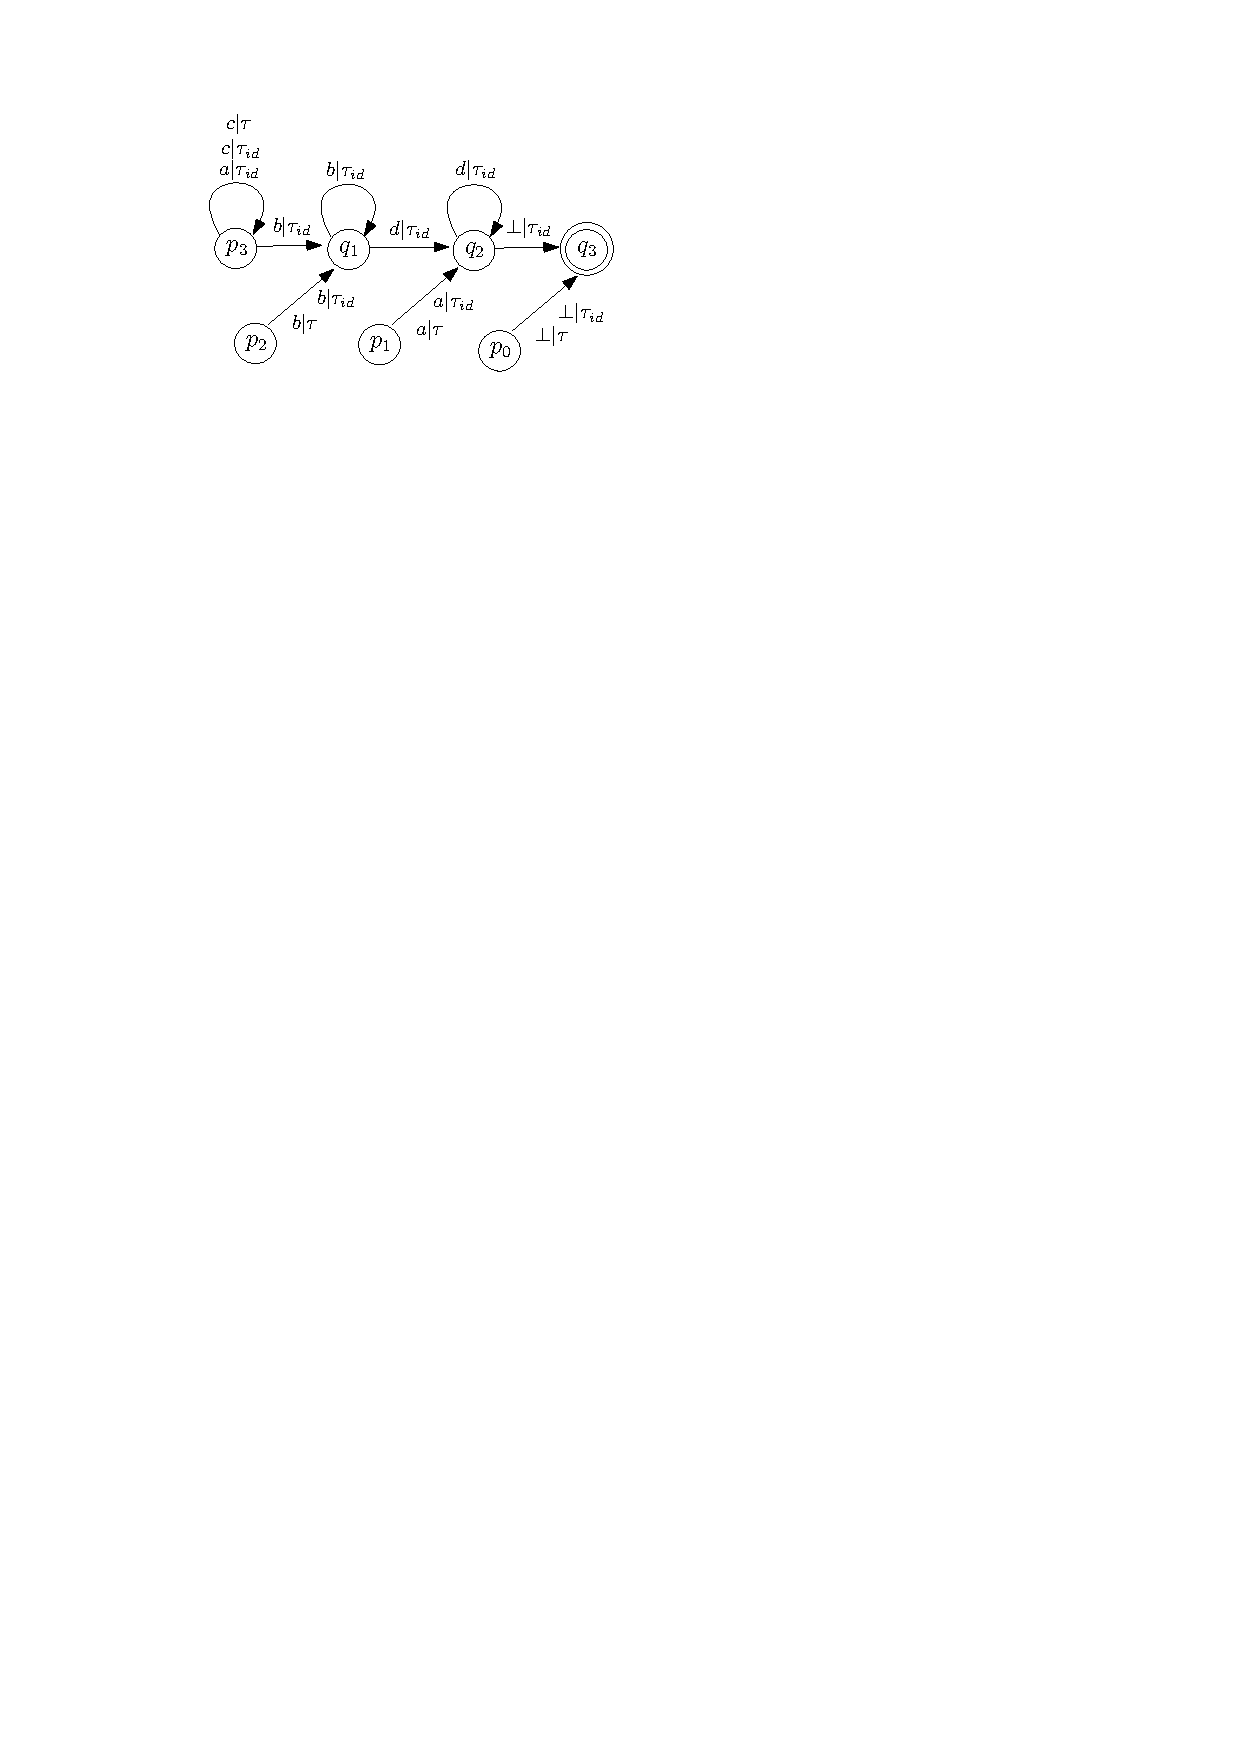
\includegraphics[scale = 0.9]{saturation-example.pdf}
	\caption{The $\Pp$-{\WOTrNFA} $\Aut^{\pre*}_{\Pp}$}\label{fig-saturation-exmp}
\end{figure}
\qed
\end{example}

Given the {\WOTrPDS} $\Pp= (P, \Gamma, \TranSet, \Delta)$, $p_1, p_2 \in P$, and two regular languages $L_1, L_2$ represented by {\NFA}s $\Aut_1 = (Q_1, \Gamma, \delta_1, I_1, F_1)$ and $\Aut_2 = (Q_2, \Gamma, \delta_2, I_2, F_2)$ respectively, the regular reachability problem is reduced to the intersection problem of the $\Pp$-{\WOTrNFA} $(\Aut_1'(p_1))^{\post*}_{\Pp}(p_2)$ and the $\Pp$-{\NFA} $\Aut_2(p_2)$, 
i.e., checking $\Lang((\Aut_1'(p_1))^{\post*}_{\Pp}(p_2)) \cap \Lang(\Aut_2(p_2)) \neq \emptyset$, where $\Aut_1' = (Q_1, \Gamma, \delta_1', I_1, F_1)$ and $\delta_1' = \{(p,\gamma,\tau_{\id}, p')\mid (p,\gamma,p')\in\delta_1\}$.
% where $\Aut_1[p_1]$ is obtained from $\Aut_1$ by adding a transition $(p_1, a, q)$ for each $(q_0, a, q) \in \delta_1$ with $q_0 \in I_1$, similarly for $\Aut_2[p_2]$. 
Then Theorem~\ref{thm-wstrpds-reach} follows from Proposition~\ref{prop-wstrnfa-nfa-intersect} in the next subsection.

%Here when we add a transition $(p,\gamma,\tau'',p')$ into $\Aa$, if there exists a transition $(p, \gamma,\tau',p')$ in the current automaton, we modify the transition $(p,\gamma,\tau',p')$ to $(p,\gamma,\tau'\cup\tau'',p')$ instead of adding $(p,\gamma,\tau'',p')$.


\subsubsection{The intersection problem of {\WOTrNFA} and {\NFA}} \label{sec:fatrnfa}
%\begin{definition}[{\WOTrNFA}-{\NFA} intersection problem]
The {\WOTrNFA}-{\NFA} intersection problem is, for given $\Pp$-{\WOTrNFA} $\Aut$ and $\Pp$-{\NFA} $\AutB$, to decide  whether $\Lang(\Aut) \cap \Lang(\AutB) = \emptyset$. We shall show that this problem %the {\WOTrNFA}-{\NFA} intersection problem to 
can be reduced to (polynomially many) instances of the sub-covering problem of a downward-WSTS, which is decidable by Theorem~\ref{thm-dwsts}.
%\end{definition}

%The rest of this section is devoted to the proof of the following result.
\begin{proposition}\label{prop-wstrnfa-nfa-intersect}
	The {\WOTrNFA}-{\NFA} intersection problem is decidable.
\end{proposition}

%For technical convenience, we define another partial order $\preceq$ on $\langle \TranSet \rangle$ as follows: $\tau_1 \preceq \tau_2$ if $\tau_1 \supseteq \tau_2$. Moreover, we use $\tau_1 \prec \tau_2$ to denote $\tau_1 \supset \tau_2$ (i.e. $\tau_1 \supseteq \tau_2$ but $\tau_1 \neq \tau_2$).

%From the fact that $(\langle \TranSet \rangle, \subseteq)$ is dually well-ordered, namely, it satisfies the ACC condition and contains no infinite antichain, we deduce that $(\langle \TranSet \rangle, \preceq)$ is well-ordered, namely, it satisfies the DCC condition and contains no infinite antichain.

%$(\langle \TranSet \rangle, \preceq)$ is well-ordered


%In the sequel, we are going to prove Proposition~\ref{prop-wstrnfa-nfa-intersect} by reducing 

%Its proof relies on the decidability of the sub-covering problem of downward-WSTS (\cite{FS01}).
% $(T, \rightarrow, \preceq)$.

\begin{proof}
%Let us fix a {\WOTrPDS} $\Pp = (P, \Gamma, \TranSet, \Delta)$, 
Assume a $\Pp$-{\WOTrNFA} $\Aut = (Q, \Gamma, \delta, I, F)$ and a $\Pp$-{\NFA} $\AutB = (Q', \Gamma, \delta', I', F')$.
We construct a downward-WSTS $\wstsnodes_{\Aut,\AutB} = (S, \rightarrow, \preceq)$ 
%
%The basic idea of $\wstsnodes_{\Aut,\AutB}$ is 
to simulate the synchronized runs of $\Aut$ and $\AutB$, where
\begin{itemize}
	\item $S = Q \times \Tranbasis \times Q'$, (Intuitively, $(q, \beta, q') \in S$ means that the current states of $\Aut$ and $\AutB$ are $q$ and $q'$ respectively, and $\beta$ is the transduction to be applied to the remaining suffix of the input string.)
	%
	\item the transition relation $\xrightarrow{}$ is defined as follows:  for every state $(q_1, \beta_1, q'_1)$ in $S$ and transition rules $(q_1, b, \beta, q_2) \in \delta$ and $(q'_1, a, q'_2) \in \delta'$, suppose that a $\Tranbasis$-representation of $( \lceil a, b \rfloor^{-1} \beta_1) \circ \beta$ is $\beta'_1 \cup \cdots \cup \beta'_k$,  then we have $(q_1, \beta_1, q'_1) \xrightarrow{} (q_2, \beta'_i, q'_2)$ for every $i \in [k]$, (Intuitively, $b$ is obtained from $a$ by applying the transduction $\beta_1$.)
%	
%	 and $(q_2, \tau_2, q'_2)$ in $ S$, $(q_1, \tau_1, q'_1) \rightarrow (q_2, \tau_2, q'_2)$ iff $\tau_1 \neq \emptyset$, and there are $a, b \in \Gamma_\varepsilon$ and a transduction $\tau$ such that $(q_1, b, \tau, q_2) \in \delta$, $(q'_1, a, q'_2) \in \delta'$, and $\tau_2 =( \lceil a, b \rfloor^{-1} \tau_1) \circ \tau$, 
	%
	\item for states $(q_1, \beta_1, q'_1)$ and $(q_2, \beta_2, q'_2)$ in $S$, $(q_1, \beta_1, q'_1) \preceq (q_2, \beta_2, q'_2)$ iff $q_1= q_2$, $q'_1 = q'_2$, and $\beta_1 \preceq \beta_2$.
\end{itemize}

To show that $\wstsnodes_{\Aut,\AutB} = (S, \rightarrow, \preceq)$ is a downward-WSTS, we first observe that $(S, \preceq)$ is a wpo since $(\Tranbasis, \preceq)$ is a wpo. Moreover, we shall show that $\rightarrow$ is downward reflexive-compatible with respect to $\preceq$. Namely, if $(q_1, \beta_1, q'_1) \rightarrow (q_2, \beta_2, q'_2)$ and $(q_1, \beta_1, q'_1) \succeq (q_3, \beta_3, q'_3)$, then there is $(q_4, \beta_4, q'_4)$ such that $(q_3, \beta_3, q'_3) \rightarrow (q_4, \beta_4, q'_4)$ and $(q_2, \beta_2, q'_2) \succeq (q_4, \beta_4, q'_4)$. 

From $(q_1, \beta_1, q'_1) \rightarrow (q_2, \beta_2, q'_2)$, there are $a, b \in \Gamma_\varepsilon$ and $\beta \in \Tranbasis$ such that $(q_1, b, \beta, q_2) \in \delta$, $(q'_1, a, q'_2) \in \delta'$, and $\beta_2$ occurs as a disjunct in a $\Tranbasis$-representation of $( \lceil a, b \rfloor^{-1} \beta_1) \circ \beta$. 

From $(q_1, \beta_1, q'_1) \succeq (q_3, \beta_3, q'_3)$, we have that $q_1 = q_3$, $q'_1 = q'_3$, and $\beta_3 \preceq \beta_1$. Therefore, $ ( \lceil a, b \rfloor^{-1} \beta_3) \circ \beta \preceq ( \lceil a, b \rfloor^{-1} \beta_1) \circ \beta$. Furthermore, since $\beta_2 \subseteq ( \lceil a, b \rfloor^{-1} \beta_1) \circ \beta $, we have $( \lceil a, b \rfloor^{-1} \beta_1) \circ \beta  \preceq \beta_2$. Then $ ( \lceil a, b \rfloor^{-1} \beta_3)  \circ \beta \preceq \beta_2$. From the distributivity of $\preceq$ over $\Tranbasis$-representations, we know that there is a disjunct $\beta_4$ of a $\Tranbasis$-representation of $( \lceil a, b \rfloor^{-1} \beta_3)  \circ \beta$ such that $\beta_4 \preceq \beta_2$.
Let $q_4 = q_2$ and $q'_4= q'_2$. Then $(q_1, \beta_3, q'_1) \rightarrow (q_2, \beta_4, q'_2)=(q_4, \beta_4, q'_4)$ and $(q_2, \beta_2, q'_2) \succeq (q_4, \beta_4, q'_4)$.

%From $(q_1, \beta_1, q'_1) \succeq (q_3, \beta_3, q'_3)$, we know that $q_1 = q_3$, $q'_1 = q'_3$, and $\beta_1 \subseteq \beta_3$.  Therefore, $\beta_2 = ( \lceil a, b \rfloor^{-1} \beta_1) \circ \tau \subseteq ( \lceil a, b \rfloor^{-1} \beta_3) \circ \tau = \beta_4$. We deduce that $\tau_2 \succeq \tau_4$ and $(q_2, \tau_2, q'_2) \succeq (q_4, \tau_4, q'_4)$. 

Therefore, $\rightarrow$ is downward reflexive-compatible with respect to $\preceq$. Furthermore, we show that $\wstsnodes_{\Aut,\AutB}$ has effective $\Succ$ and decidable $\preceq$.
\begin{itemize}
	%\item Since $(\wstsnodes_{\Aut,\AutB}, \rightarrow, \preceq)$ has strong downward-compatibility, it follows that it also has reflexive downward-compatibility.
	%
	\item Given a state $(q_1, \beta_1, q'_1)$, $\Succ((q_1, \beta_1, q'_1))$ can be computed effectively as follows: Enumerate all the pairs of transition rules $(q_1, b, \beta, q_2) \in \delta$ (there are only finitely many of them) and $(q'_1, a, q'_2) \in \delta'$, and for every such pair of transitions, compute a $\Tranbasis$-representation of $( \lceil a, b \rfloor^{-1} \beta_1) \circ \beta$, say $\beta'_1 \cup \cdots \cup \beta'_k$, then for each $i \in [k]$, put $(q_2, \beta'_i, q'_2)$ into $\Succ((q_1, \beta_1, q'_1))$.
	%
	\item Finally, given two states $(q_1, \tau_1, q'_1)$ and $(q_2, \tau_2, q'_2)$ (where $\tau_1, \tau_2$ are given as {\NFT}s), from Proposition~\ref{prop-nft-inclusion}, we can effectively decide whether $\tau_1 \preceq \tau_2$, namely, $\tau_2 \subseteq \tau_1$. Therefore, $\wstsnodes_{\Aut,\AutB}$ has decidable $\preceq$.
\end{itemize}

Then $\Lang(\Aut) \cap \Lang(\AutB) \neq \emptyset$ iff $p \xRightarrow{w | \tau} q$, $p' \xRightarrow{w} q'$, and $(\varepsilon, \varepsilon) \in \tau$ for some $p \in I$, $p'\in I'$, $w \in \Gamma^*$, $\tau \in \langle \TranSet \rangle$, $q \in F$, and $q' \in F'$. Suppose that a $\Tranbasis$-representation of $\tau_{id}$ is $\beta_1 \cup \cdots \cup \beta_k$. 
The construction of $\wstsnodes_{\Aut,\AutB}$ entails that $p \xRightarrow{w | \tau} q$, $p' \xRightarrow{w} q'$, and $(\varepsilon, \varepsilon) \in \tau$ for some $w \in \Gamma^*$  and $\tau \in \langle \TranSet \rangle$  iff $(q, \beta', q')$ is reachable from $(p, \beta_i, p')$ in $\wstsnodes_{\Aut,\AutB}$ and $\beta' \preceq \tau_\varepsilon$ for some $\beta' \in \Tranbasis$ and $i \in [k]$, where $\beta'$ occurs as a disjunct of a $\Tranbasis$-representation of $\tau$. 
%
Furthermore, $(q, \beta', q')$ is reachable from $(p, \beta_i, p')$ in $\wstsnodes_{\Aut,\AutB}$ and $\beta' \preceq \tau_\varepsilon$ for some $\beta' \in \Tranbasis$ and $i \in [k]$ iff $(q, \beta', q')$ is reachable from $(p, \beta_i, p')$ in $\wstsnodes_{\Aut,\AutB}$ and $(q, \beta', q')$ sub-covers $(q, \tau_\varepsilon, q')$ for some $\beta' \in \Tranbasis$ and $i \in [k]$. Therefore, we deduce that \emph{$\Lang(\Aut) \cap \Lang(\AutB) \neq \emptyset$ iff there are $p \in I$, $p' \in I'$, $q \in F$, $q' \in F'$, and $i \in [k]$ such that starting from $(p, \beta_i, p')$, a state that sub-covers $(q, \tau_\varepsilon, q')$ can be reached}.
%\end{quote}
We conclude from Theorem~\ref{thm-dwsts} that the {\WOTrNFA}-{\NFA} intersection problem is decidable.
\end{proof}


\subsection{Solving the configuration reachability problem of $\singletask$-dominating $\IFAMASS$}\label{sec-ifamass-reach}

From the definition of the configuration reachability problem in Section~\ref{sec-conf-reach}, for the $\singletask$-dominating $\IFAMASS$ $\Mm$, we should solve the following problem: given an {\NFA} $\Aa' = (Q', \act, \delta', I', F')$ over the alphabet $\act$, decide whether $\confs((\aft(A_0), \Aa')) \cap \RConfs(\Mm) \neq \emptyset$. 

While it is relatively easy to simulate the operations $\POP, \PUSH, \STP, \CTP$, %by the transition rules of $\Pp_\Aut$, 
it is challenging to  simulate $\RTF$. The semantics of $A \xrightarrow{\startactivity(\phi)}B$ such that $\phi \models \neg \ctpflag \wedge \rtfflag$ requires to move the topmost occurrence of $B$ (if there is any) to the top of the stack. The most direct way to simulate  $A \xrightarrow{\startactivity(\phi)}B$ such that $\phi \models \neg \ctpflag \wedge \rtfflag$ ans $A \neq B$ is by two transition rules $p \xrightarrow{A / B | \tau_{B, A}} p$ and  $p \xrightarrow{A / BA | \tau_{\not B}} p$
%\jl{this should be $p \xrightarrow{A / BA | \tau_{\not B}} p$}
(where $p$ is a state in $\Pp_\Aut$), corresponding to the two situations that $B$ occurs/does no occur in the stack, where 
\begin{itemize}
\item $\tau_{B, A}$ is the transduction that removes the first occurrence of $B$ from the input string and adds $A$ in the beginning, and
%
\item $\tau_{\not B}$ checks that $B$ does not occur in the input string but keeps the input string unchanged. 
\end{itemize}

%Our idea is to ues {\WOTrPDS} $\Pp_{\Mm}$ to simulate the behaviors fo $\Mm$, recall that we use $\tau_{B, A}$ to simulate $A\xrightarrow{\startactivity(\phi_{\rtfflag})}B$ with $\phi_{\rtfflag}\models\rtfflag\wedge\neg\ctpflag$.

However, such a direct simulation would entail an \emph{infinite} antichain in the transduction closure: $\tau^n_{B, A}$  (where $n \ge 1$), i.e. the $n$-fold composition of $\tau_{B,A}$, is the transduction that removes the first $n$ occurrences of $B$ from the input string and add $n$ $A$'s in the beginning. It is easy to observe that for every $i, j$ with $i \neq j$, $\tau^i_{B, A}$ and $\tau^j_{B, A}$ are incomparable with respect to $\preceq$, namely, neither $\tau^i_{B, A} \subseteq \tau^j_{B, A}$, nor $\tau^j_{B, A} \subseteq \tau^i_{B, A}$. Therefore, $\tau_{B, A}, \tau^2_{B, A}, \tau^3_{B, A}, \cdots$ comprises an infinite antichain with respect to $\preceq$. 

To ensure that the transduction closure of $\Pp_\Mm$  has a well-partially-ordered union-basis, we
apply the following tricks: when simulating $A \xrightarrow{\startactivity(\phi)}B$ such that $\phi \models \neg \ctpflag \wedge \rtfflag$ and $A \neq B$,
\begin{itemize}
\item instead of moving the first occurrence of $B$ to the beginning of the input string, we replace the first occurrence of $B$ with a dummy symbol $\dag$ and push $B$ into the stack, and
%
\item $A \xrightarrow{\startactivity(\phi)}B$ is simulated by the transition rules $p \xrightarrow{A / BA | \tau_{B, \dag}} p$ and  $p \xrightarrow{A / BA | \tau_{\not B}} p$, where $\tau_{B, \dag}$ is the transduction that replaces \emph{at least the first occurrence of $B$ with $\dag$}. More precisely, $\tau_{B, \dag}$ nondeterministically chooses some $n \ge 1$ and replaces each of the first $n$ occurrences of $B$ with $\dag$.
\end{itemize}
%\tl{revisit here}
The aforementioned tricks are justified by the observation that the transition $A \xrightarrow{\startactivity(\phi)}B$ such that $\phi \models \neg \ctpflag \wedge \rtfflag$ and $A \neq B$ could be continuously applied for multiple times: Namely, when the topmost occurrence of $B$ is moved to the top of the stack, $B$ can be popped and $A$ becomes the top activity of the stack again. Then the transition $A \xrightarrow{\startactivity(\phi)}B$ can be applied for the second time to move the top second occurrence of $B$  (referring to the original contents of the stack) to the top. Furthermore, this process can be continued if there are still some occurrences of $B$ in the stack. Therefore, the simulation of $A \xrightarrow{\startactivity(\phi)}B$ such that $\phi \models \neg \ctpflag \wedge \rtfflag$ and $A \neq B$ by $p \xrightarrow{A / BA | \tau_{B, \dag}} p$ and  $p \xrightarrow{A / BA | \tau_{\not B}} p$ is sound in the sense that it does \emph{not} introduce unreachable configurations.

%We first show that a  {\ASS} $\Aut = (Act, A_0,\Delta)$ can be simulated by a pushdown system with transductions $\Pp_\Aut = (P_\Aut, \Gamma_\Aut, \TranSet_\Aut, \Delta_\Aut)$. Then we prove that $(\langle \TranSet_\Aut \rangle, \preceq)$ is well-ordered, that is, $\Pp_\Aut$ is a {\WOTrPDS}. The decidability of the configuration reachability problem of {\ASS} then follows from Theorem~\ref{thm-wstrpds-reach}.

\paragraph*{From $\Mm$ to $\Pp_\Mm$} 
The {\WOTrPDS} $\Pp_\Mm = (P_\Mm, \Gamma_\Mm, \TranSet_\Mm, \Delta_\Mm)$ where 
\begin{itemize}
\item $P_{\Mm} = \{p_0\}\cup\{ p_{B}\mid B\in\act\}$,
\item $\Gamma_{\Mm} = \act \cup \{\dag\}$, 
\item $\TranSet_\Mm = \{\tau_{\id} \}\cup \{\tau_{B, \dag} \mid B \in \act\} \cup \{\tau_{B} \mid B \in \act\}  \cup \{\tau_{\not B} \mid B \in \act\}$, where $\tau_B$ is the transduction that checks that $B$ occurs in the input string but keeps the input string unchanged, and 
\item $\Delta_{\Mm}$ is defined as follows:
        \begin{itemize}
            \item for each $A \in \act$, $(p_0, A, \varepsilon, \tau_{\id}, p_0) \in \Delta_{\Mm}$, (Recall that $\back$ can be applied anytime in $\Mm$.)
			\item for each transition $A \xrightarrow{\startactivity(\phi)} B$, 
			\begin{itemize}
				\item if $\phi \models \ctpflag$ and $A \neq B$, then $(p_0, A, BA, \tau_{\not B}, p_0) \in \Delta_{\Mm}$, $(p_0, A, \varepsilon, \tau_{B}, p_B) \in \Delta_{\Mm}$, $(p_B, B, B, \tau_{\id}, p_0)  \in \Delta_{\Mm}$, and for each $\gamma \in \Gamma_\Mm \setminus \{B\}$, $(p_B, \gamma, \varepsilon, \tau_{\id}, p_B) \in \Delta_{\Mm}$, 
%
				\item if $\phi\models \neg\ctpflag \wedge \rtfflag$ and $A \neq B$, then $(p_0, A, BA, \tau_{\not B}, p_0) \in \Delta_{\Mm}$ 
                and $(p_0, A, BA, \tau_{B, \dag}, p_0) \in \Delta_{\Mm}$,
                %
				\item if $\phi \models \neg\ctpflag \wedge \neg \rtfflag \wedge \stpflag$ and $A \neq B$, then $(p_0, A, BA, \tau_{\id}, p_0) \in \Delta_{\Mm}$,
%
				\item if $\phi \models \neg\ctpflag \wedge \neg \rtfflag \wedge \neg \stpflag$, then $(p_0, A, BA, \tau_{\id}, p_0) \in \Delta_{\Mm}$.
			\end{itemize}
            %
        \end{itemize}
\end{itemize}
%$\tau_{\CTK} = (\{p_0, q_f\}, \Gamma \cup \{\dag, \bot\}, \delta_{\CTK}, p_0, \{q_f\})$, where $\delta_{\CTK}$ is defined as follows.
%\begin{itemize}
%    \item for each $\gamma \in \Gamma \cup \{\dag\}$, we have $(p_0, \gamma, \dag, p_0) \in \delta_{\CTK}$,
%    \item we have $(p_0, \bot, \bot, q_f) \in \delta_{\CTK}$.
%\end{itemize}
%Intuitively, $\tau_{\CTK}$ transduces $w\bot$ into $\dag^{|w|}\bot$.

%\zhilin{stopped here}


If we know that $\Pp_\Mm$ constructed above is a {\WOTrPDS}, then the problem of deciding whether $\confs((\aft(A_0), \Aa')) \cap \RConfs(\Mm) \neq \emptyset$ is reduced to the regular reachability problem of $\Pp_\Mm$, that is, decide whether $\Lang(\Aa'')  \cap \Lang((\Aut_{A_0})^{\post^*}_{\Pp_{\Mm}}(p_0)) \neq \emptyset$, where $\Aa''$ is obtained from $\Aa'$ by adding the transitions $(q, \dag, q)$ for every $q \in Q'$ and $\Aut_{A_0}$ is the {\WOTrNFA} recognizing the set of initial configurations, i.e. $\Aut_{A_0} = (P_\Mm \cup \{p_f\}, \Gamma_{\Mm}, \{(p_0, A_0, \tau_{\id}, p_f)\}, \{p_0\}, \{p_f\})$. 

%Let $\Aut_{A_0} = (P_\Mm \cup \{p_f\}, \Gamma_{\Mm}, \{(p_0, A_0, \tau_{\id}, p_f)\}, \{p_0\}, \{p_f\})$ be a $\Pp_{\Mm}$-$\WOTrNFA$, and $\Aut = (Q, \act, \delta, I, F)$ be an $\NFA$ over the alphabet $\act$, 
%then the configuration reachability problem of $\Mm$ is solved as follows:  If $\ConfSet((\Aut_{A_0})^{\post^*}_{\Pp_{\Mm}})\cap \ConfSet(\Aut') \neq \emptyset$, where $\Aut'$ is obtained from $\Aut$ by adding the transitions $(q,\dag,q)$ for every $q \in Q$, then report ``yes'', otherwise, report ``no''.


It remains to show that $\Pp_\Mm$ is a {\WOTrPDS}. It is sufficient to prove the following result. 
%$\langle \TranSet_\Aut \rangle$ has a union-basis $\Tranbasis$ satisfying the four conditions in Definition~\ref{def:defatpds}.

\begin{proposition}\label{lem-transet-wo}
$\langle \TranSet_\Mm \rangle$ has a union-basis $\Tranbasis$ satisfying the four conditions in Definition~\ref{def:defatpds}.
\end{proposition}

% We now complete the proof of Theorem~\ref{thm:st-amass-reach}. For a given {\NFA} $\AutB = (Q, \act, \delta, I, F)$ over $\act$, let $\AutB'$ be the {\NFA} obtained from $\AutB$ by adding the transitions $(q, \dag, q)$ for every $q \in Q$. Then $\ConfSet(\Mm) \cap \ConfSet(\AutB) \neq \emptyset$ iff there is $w \in \ConfSet(\AutB')$ such that $(p_0, A_0) \xRightarrow{\Pp_\Mm} (p_0, w)$.
%$pre^*_{\Pp_\Aut}(\ConfSet(\AutB'[p_0])) \cap \{(p_0, A_0)\} \neq \emptyset$, where $\AutB'[p_0]$ is obtained from $\AutB'$ by adding the state $p_0$ and the transitions $(p_0, a, q)$ for all $(p, a, q) \in \delta$ with $p \in I$. 

%From Theorem~\ref{thm-wstrpds-reach}, we conclude that Theorem~\ref{thm:st-amass-reach} holds.

The rest of this section is devoted to the proof of Proposition~\ref{lem-transet-wo}.
%, Proposition~\ref{prop-tranbasis-ef} and Proposition~\ref{prop-tranbasis-udist}.

%\subsection*{Proof of Proposition~\ref{lem-transet-wo}}
To prove Proposition~\ref{lem-transet-wo}, we first define $\Tranbasis_\Mm$.
For technical convenience, we fix a linear order $<$ on $\act$. Moreover, we introduce some additional notations for transductions.
\begin{itemize}
\item $\tau_\dag$ (resp. $\tau_{\not \dag}$) is the transduction that checks that $\dag$ occurs at least once (resp. $\dag$ does not occur), but keep the input string unchanged, 
%
\item $\tau_{\mathcircled{\Lambda}}$ is the transduction that checks that the set of symbols occurring in the input string is exactly $\Lambda$, %(i.e. all the symbols in the input string are from $\Lambda$ and each symbol in $\Lambda$ occurs in the input string), 
but keeps the input string unchanged. 
\end{itemize}

We then define $\Tranbasis_\Mm$ as the union of $\{\emptyset, \tau_\varepsilon\}$ and the set of transductions of the  form $\tau_{\dag} \circ \tau^{n_1}_{A_1, \dag} \circ \cdots \circ \tau^{n_k}_{A_k, \dag} \circ \tau_{\mathcircled{\Lambda}}$ or $\tau_{\not \dag} \circ \tau^{n_1}_{A_1, \dag} \circ \cdots \circ \tau^{n_k}_{A_k, \dag} \circ \tau_{\mathcircled{\Lambda}}$ such that 
1) $A_i \in \act$ and $n_i \ge 1$ for every $i \in [k]$, 
2) $A_1 < \cdots < A_k$ (which implies that they are distinct), 
3) $\Lambda \subseteq \Gamma_\Mm$ is nonempty. Note that here it is possible that $k=0$.

It remains to show that $\Tranbasis_\Mm$ satisfies the four conditions in Definition~\ref{def:defatpds}.

First, by the definition of $\Tranbasis_\Mm$, we have that $\{\emptyset, \tau_{\varepsilon}\} \subseteq \Tranbasis_\Mm$.

To show that $(\Tranbasis_\Mm, \preceq)$ is a wpo, it is sufficient to show that for every $k > 0$, $A_1 < \cdots < A_k$, and $\emptyset \neq \Lambda \subseteq \Gamma_\Mm$, the set of transductions of the form $\tau_{\alpha} \circ \tau^{n_1}_{A_1, \dag} \circ \cdots \circ \tau^{n_k}_{A_k, \dag} \circ \tau_{\mathcircled{\Lambda}}$  is a wpo (where $\alpha \in \{\dag, \not \dag\}$).  
%
It is easy to observe that if $\tau_{\alpha} \circ \tau^{n_1}_{A_1, \dag} \circ \cdots \circ \tau^{n_k}_{A_k, \dag} \circ \tau_{\mathcircled{\Lambda}} \neq \emptyset$ and $\tau_{\alpha} \circ \tau^{n'_1}_{A_1, \dag} \circ \cdots \circ \tau^{n'_k}_{A_k, \dag} \circ \tau_{\mathcircled{\Lambda}} \neq \emptyset$, 
then 
$\tau_{\alpha} \circ \tau^{n_1}_{A_1, \dag} \circ \cdots \circ \tau^{n_k}_{A_k, \dag} \circ \tau_{\mathcircled{\Lambda}} \preceq \tau_{\alpha} \circ \tau^{n'_1}_{A_1, \dag} \circ \cdots \circ \tau^{n'_k}_{A_k, \dag} \circ \tau_{\mathcircled{\Lambda}}$ iff $\tau_{\alpha} \circ \tau^{n_1}_{A_1, \dag} \circ \cdots \circ \tau^{n_k}_{A_k, \dag} \circ \tau_{\mathcircled{\Lambda}} \supseteq \tau_{\alpha} \circ \tau^{n'_1}_{A_1, \dag} \circ \cdots \circ \tau^{n'_k}_{A_k, \dag} \circ \tau_{\mathcircled{\Lambda}}$ iff $n_1 \le n'_1$, $\cdots$, and $n_k \le n'_k$. According to Dickson's lemma \cite{Kruskal72,Milner1985},  $(\Nat^k, \leq)$ is a wpo. We deduce that  $(\Tranbasis_\Mm, \preceq)$ is a wpo.

The verification of the third and fourth conditions in Definition~\ref{def:defatpds} for $\Tranbasis_\Mm$ is given by the following two propositions.

\begin{proposition}\label{prop-tranbasis-ef}
For each $\tau \in \langle \TranSet_\Mm \rangle$, a $\Tranbasis_\Mm$-representation $\beta_\tau$ can be computed effectively.
\end{proposition}

\begin{proposition}\label{prop-tranbasis-udist}
$\preceq$ is union-distributive over $\Tranbasis_\Mm$-representations.
\end{proposition}


%\subsection*{Proof of Proposition~\ref{prop-tranbasis-ef}}
\begin{proof}[Proposition~\ref{prop-tranbasis-ef}]
	We prove by a structural induction on the definition of $\langle \TranSet_\Mm \rangle$.
	
%	We first notice that every finite union of {\UFNF} $\beta_1 \cup \cdots \cup \beta_m$ can be turned into an {\AUNF} $\beta'_1 \cup \cdots \cup \beta'_n$, where $\beta'_1, \cdots, \beta'_n$ are antichains, by iterating the following process until no more {\UFNF} can be removed: if $\beta_i \preceq \beta_j$ (that is, $\beta_j \subseteq \beta_i$),  we remove $\beta_j$. Therefore, in the proof below, to show   $\beta_1 \cup \cdots \cup \beta_m$ is an {\AUNF}, we only need to show (i) in Definition~\ref{def-nf}.
	%ignore the requirement that $\beta_1, \cdots, \beta_m$ are antichains.
	
	\smallskip
	\noindent \emph{Base case.} We show that $\tau_{id}$ and all $\tau_{B}$, $\tau_{\not B}$, and $\tau_{B, \dag}$ for $B \in \act$ can be rewritten as $\Tranbasis_\Mm$-representations.
	%
	\begin{itemize}
	\item $\tau_{id} = \bigcup\limits_{\emptyset \neq \Lambda  \subseteq\Gamma_{\Mm}} (\tau_\dag \circ \tau_{\Lambda} \cup \tau_{{\not \dag}} \circ \tau_{\Lambda})$, 
	%
	\item $ \tau_{B} = \bigcup\limits_{ \Lambda \subseteq\Gamma_{\Mm}, B \in \Lambda} (\tau_\dag \circ \tau_{\Lambda} \cup \tau_{{\not \dag}} \circ \tau_{\Lambda}),$
	% \cup \left(\bigcup\limits_{\Lambda \subseteq \Gamma_{\Aut}\setminus \{\dag\}, B \in \Lambda} \tau_{\not \dag} \circ \tau_{\Lambda}\right),$$  
	%
	\item	$ \tau_{\not B} =
	\bigcup\limits_{\emptyset \neq \Lambda \subseteq\Gamma_{\Mm}, B \not \in \Lambda} (\tau_\dag \circ \tau_{\Lambda} \cup \tau_{\not \dag} \circ \tau_{\Lambda}),$  
	%
	\item $\tau_{B,\dag} = \bigcup\limits_{\emptyset \neq \Lambda \subseteq \Gamma_{\Mm}}(\tau_{\dag} \circ \tau_{B,\dag}^1\circ\tau_{\Lambda} \cup \tau_{\not \dag} \circ \tau_{B,\dag}^1\circ\tau_{\Lambda} )$.
	%
%	$\emptyset =\tau_\dag \circ \tau_{\{A\}}$ for every $A \in Act$. 
	%Note that the composition of $\tau_{A,\dag}^1$ and  $\tau_{\{A\}}$ is equal to $\emptyset$, since $\tau_{A,\dag}^1$ implies that $\dag$ must occur in the output string of $\tau_{A,\dag}^1$, while $\tau_{\{A\}}$ requires that $\dag$ does not occur.
	%
%	\item $\tau_{\id} = \bigcup\limits_{\emptyset \neq \Lambda \subseteq \Gamma_{\Aut}}(\tau_\dag \circ \tau_{\Lambda} \cup \tau_{\not \dag} \circ \tau_\Lambda)$.
	\end{itemize}
	
	For the induction step, we show the following claim. 
	
	\noindent \emph{Claim. Suppose that $\beta_1, \beta_2 \in \Tranbasis_\Mm$ and $\gamma, \gamma' \in \Gamma_\Mm$. Then $\beta_1 \circ \beta_2$ and $\lceil \gamma, \gamma' \rfloor^{-1}\beta_1$ can be rewritten into $\Tranbasis_\Mm$-representations.}
	
	\smallskip
	
	\noindent \emph{Proof of the claim.}
	%
	We consider $\beta_1 \circ \beta_2$ first.
	%

	Suppose that $\beta_1 = \tau_{\alpha_1} \circ \tau^{n_{1,1}}_{A_{1,1}, \dag} \circ \cdots \circ \tau^{n_{1, k_1}}_{A_{1,k_1}, \dag} \circ \tau_{\mathcircled{\Lambda_1}}$ and $\beta_2 = \tau_{\alpha_2} \circ \tau^{n_{2,1}}_{A_{2,1}, \dag} \circ \cdots \circ \tau^{n_{2, k_2}}_{A_{2,k_2}, \dag} \circ \tau_{\mathcircled{\Lambda_2}}$, where $\alpha_1, \alpha_2 \in \{\dag, \not \dag\}$.
	
	If $\beta_1 \circ \beta_2 = \emptyset$, then $\emptyset$ is already a $\Tranbasis_\Mm$-representation of $\beta_1 \circ \beta_2$. 
	
	Below we assume that $\beta_1 \circ \beta_2 \neq \emptyset$. This implies that $\beta_1 \neq \emptyset$ and $\beta_2 \neq \emptyset$.
	% 
	We exemplify the proof for the case that $\alpha_1 = {\not \dag}$ and  $\alpha_2 = \dag$.
	
	In this case, $\Lambda_1 =  \{A_{2,1}, \cdots, A_{2, k_2}\} \cup \Lambda_2$. The arguments proceed as follows. 
	Each symbol in the outputs of $\beta_1$ must be either in $\{A_{2,1}, \cdots, A_{2, k_2}\}$ or in $\Lambda_2$, i.e., $\Lambda_1 \subseteq   \{A_{2,1}, \cdots, A_{2, k_2}\} \cup \Lambda_2$. On the other hand, all the symbols in $\{A_{2,1}, \cdots, A_{2, k_2}\} \cup \Lambda_2$, except $\dag$, must occur in the inputs of $\beta_2$, namely, the outputs of $\beta_1$, thus  $(\{A_{2,1}, \cdots, A_{2, k_2}\} \cup \Lambda_2) \setminus \{\dag\} \subseteq \Lambda_1$.
	Therefore, we have that
	$(\{A_{2,1}, \cdots, A_{2, k_2}\} \cup \Lambda_2) \setminus \{\dag\} \subseteq \Lambda_1 \subseteq  \{A_{2,1}, \cdots, A_{2, k_2}\} \cup \Lambda_2$, that is, $\Lambda_1 = (\{A_{2,1}, \cdots, A_{2, k_2}\} \cup \Lambda_2) \setminus \{\dag\}$ or $\Lambda_1 =  \{A_{2,1}, \cdots, A_{2, k_2}\} \cup \Lambda_2$.
	%
	Moreover, $\alpha_2 = \dag$, and thus $\dag \in \Lambda_1$. Hence  $\Lambda_1 =  \{A_{2,1}, \cdots, A_{2, k_2}\} \cup \Lambda_2$.
	%
	%If $\Lambda_1 = (\{A_{2,1}, \cdots, A_{2, k_2}\} \cup \Lambda_2) \setminus \{\dag\}$, then $k_1 = 0$ (otherwise, $\dag \in \Lambda_1$). 
	%
	%Since $\beta_2 \neq \emptyset$ implies that all the symbols in $\{A_{2,1}, \cdots, A_{2, k_2}\} \cup \Lambda_2$, except $\dag$, must occur in the input strings of $\beta_2$,  we deduce that 
	%$$\beta_1 \circ \beta_2 = \tau_{\not \dag} \circ \tau_{\Lambda_1} \circ \beta_2 = 
	%\tau_{\not \dag} \circ \tau^{n_{2,1}}_{A_{2,1}, \dag} \circ \cdots \circ \tau^{n_{2, k_2}}_{A_{2,k_2}, \dag} \circ \tau_{\mathcircled{\Lambda_2}}.$$
	%
	
	Furthermore, we have $k_1 > 0$ because otherwise $\beta_1 = \tau_{\not \dag} \circ \tau_{\Lambda_1} = \emptyset$, contradicting the assumption that $\beta_1 \circ \beta_2 \neq \emptyset$. 
	%
	%$\beta_1 \circ \beta_2 = \tau_{\not \dag} \circ \tau_{\Lambda_1} \circ \beta_2 = 
	%\tau_{\dag} \circ \tau^{n_{2,1}}_{A_{2,1}, \dag} \circ \cdots \circ \tau^{n_{2, k_2}}_{A_{2,k_2}, \dag} \circ \tau_{\mathcircled{\Lambda_2}}$.
	%
	%Since $k_1 > 0$, we do not know for sure that $\dag$ occurs in the input strings of $\beta_1$. Therefore, 
	Consequently, 
	%
	$$\beta_1 \circ \beta_2 = 
	%\tau_{\dag} \circ \tau^{n'_{1}}_{A'_{1}, \dag} \circ \cdots \circ \tau^{n'_{k'}}_{A'_{k'}, \dag} \circ \tau_{\mathcircled{\Lambda_2}}\ \cup\ 
	\tau_{\not \dag} \circ \tau^{n'_{1}}_{A'_{1}, \dag} \circ \cdots \circ \tau^{n'_{k'}}_{A'_{k'}, \dag} \circ \tau_{\mathcircled{\Lambda_2}},$$
	%
	%
	where $\tau^{n'_{1}}_{A'_{1}, \dag} \circ \cdots \circ \tau^{n'_{k'}}_{A'_{k'}, \dag}$ is obtained by combining 
	$ \tau^{n_{1,1}}_{A_{1,1}, \dag} \circ \cdots \circ \tau^{n_{1, k_1}}_{A_{1, k_1}, \dag}$
	and 
	$ \tau^{n_{2,1}}_{A_{2,1}, \dag} \circ \cdots \circ \tau^{n_{2, k_2}}_{A_{2,k_2}, \dag}$. More precisely, $\tau^{n'_{1}}_{A'_{1}, \dag} \circ \cdots \circ \tau^{n'_{k'}}_{A'_{k'}, \dag}$ is obtained by reordering the transductions $ \tau^{n_{1,1}}_{A_{1,1}, \dag}, \cdots, \tau^{n_{1, k_1}}_{A_{1, k_1}, \dag},  \tau^{n_{2,1}}_{A_{2,1}, \dag}, \cdots, \tau^{n_{2, k_2}}_{A_{2,k_2}, \dag}$ according to the linear order on $\act$,
	and merging $\tau^{n_{1,j_1}}_{A_{1, j_1}, \dag}$ and $\tau^{n_{2, j_2}}_{A_{2, j_2}, \dag}$, thus creating $\tau^{n_{1,j_1} + n_{2, j_2}}_{A_{1, j_1}, \dag}$, for every $j_1 \in [k_1]$ and $j_2 \in [k_2]$ such that $A_{1, j_1} = A_{2, j_2}$.  
	
	Next, let us consider $\lceil \gamma, \gamma' \rfloor^{-1} \beta_1$. 
	%
	%If $\alpha_1 = \dag$, then 
	\begin{itemize}
		%\item if $\gamma  = \dag$ and $\gamma' = \dag$, then $\lfloor \gamma, \gamma' \rceil^{-1} \beta_1 = \beta_1$,
		%
		\item If $\gamma = A_{1, j}$ and $\gamma' = \dag$ for some $j \in [k_1]$, then if $n_{1,j} \ge 2$, we have
		%
		$$\lceil \gamma, \gamma' \rfloor^{-1} \beta_1 = \tau_{ \alpha_1} \circ \tau^{n_{1,1}}_{A_{1,1}, \dag} \circ \cdots \circ \tau^{n_{1,j-1}}_{A_{1,j-1}, \dag}  \circ \tau^{n_{1,j}-1}_{A_{1,j}, \dag}  \circ  \tau^{n_{1, j+1}}_{A_{1, j+1}, \dag}  \circ \cdots \circ \tau^{n_{1, k_1}}_{A_{1, k_1}, \dag} \circ \tau_{\mathcircled{\Lambda_1}},$$ 
		%
		otherwise, $n_{1,j} = 1$, since $\lceil \gamma, \gamma' \rfloor^{-1} \tau_{A_{1,j}, \dag} = \lceil A_{1, j}, \dag \rfloor^{-1} \tau_{A_{1,j}, \dag} = \tau_{id} \cup \tau_{A_{1,j}, \dag}$,  we have
		%
		$$
		\begin{array}{l c l}
		\lceil \gamma, \gamma' \rfloor^{-1} \beta_1 & = & \tau_{\alpha_1} \circ \tau^{n_{1,1}}_{A_{1,1}, \dag} \circ \cdots \circ \tau^{n_{1,j-1}}_{A_{1,j-1}, \dag}  \circ \tau^{n_{1,j+1}}_{A_{1,j+1}, \dag} \cdots \circ \tau^{n_{1, k_1}}_{A_{1, k_1}, \dag} \circ \tau_{\mathcircled{\Lambda_1}}\ \cup  \\ 
		& & \tau_{\alpha_1} \circ \tau^{n_{1,1}}_{A_{1,1}, \dag} \circ \cdots \circ \tau^{n_{1,j-1}}_{A_{1,j-1}, \dag}  \circ \tau_{A_{1,j}, \dag}\ \cup\\
		& & \tau^{n_{1,j+1}}_{A_{1,j+1}, \dag} \cdots \circ \tau^{n_{1, k_1}}_{A_{1, k_1}, \dag} \circ \tau_{\mathcircled{\Lambda_1}}.
		\end{array}
		$$
		Therefore, in this case, $\lceil \gamma, \gamma' \rfloor^{-1} \beta_1$ can be rewritten into a $\Tranbasis$-representation.
		%%
		\item If $\gamma \in \Lambda_1 \setminus \{A_{1,1}, \cdots, A_{1, k_1}\}$ and $\gamma' = \gamma$, then $\lceil \gamma, \gamma' \rfloor^{-1} \beta_1 = \beta_1$. 
		%%
		\item For all the other cases, we have $\lceil \gamma, \gamma' \rfloor^{-1} \beta_1 = \emptyset$.
	\end{itemize}
	\qed
	
	\smallskip
	\noindent\emph{Induction step.} Assume that $\tau_1$, $\tau_2$, and $\tau$ have been rewritten into $\Tranbasis$-representations. We show that $\tau_1 \circ \tau_2$, $\tau_1 \cup \tau_2$, and $\lfloor \gamma, \gamma' \rfloor^{-1} \tau$ can be rewritten into $\Tranbasis$-representations as well.
	
	%We now complete the induction step.
	
	Case $\tau_1 \circ \tau_2$: Suppose that  $\tau_1$ and $\tau_2$ can be rewritten into the $\Tranbasis$-representations $ \beta_{1,1} \cup \cdots \cup \beta_{1, m_1}$ and $\beta_{2,1} \cup \cdots \cup \beta_{2, m_2}$  respectively.
	% where $\beta_{i, j} = \tau_{\alpha_i} \circ \tau^{n_{i, 1}}_{A_{i, 1}, \dag} \circ \cdots \circ \tau^{n_{i, k_{i,j}}}_{A_{i, k_{i,j}}, \dag} \circ \tau_{\mathcircled{\Lambda_i}}$ for every $i \in \{1,2\}$ and $j \in [m_i]$. 
	
	Then $\tau_1 \circ \tau_2$ is equivalent to $\bigcup \limits_{j_1 \in [m_1]} \bigcup \limits_{j_2 \in [m_2]} \beta_{1, j_1} \circ \beta_{2, j_2}$. From the Claim, we know that each of $ \beta_{1, j_1} \circ \beta_{2, j_2}$ can be rewritten into $\Tranbasis$-representations. Thus $\tau_1 \circ \tau_2$ can be rewritten into $\Tranbasis$-representations as well.
	
	Case $\tau_1 \cup \tau_2$: Trivial.
	
	Case $\lceil \gamma, \gamma' \rfloor^{-1} \tau$: Suppose that $\tau$ can be rewritten into a $\Tranbasis$-representation $ \beta_{1} \cup \cdots \cup \beta_{m}$. 
	%where $\beta_{j} = \tau_{\alpha} \circ \tau^{n_{1}}_{A_{1}, \dag} \circ \cdots \circ \tau^{n_{ k_{j}}}_{A_{k_{j}}, \dag} \circ \tau_{\mathcircled{\Lambda}}$ for every $j \in [m]$. 
	Then $\lceil \gamma, \gamma' \rfloor^{-1} \tau = \bigcup \limits_{j \in [m]} \lceil \gamma, \gamma' \rfloor^{-1} \beta_j$. From the claim, each of $\lceil \gamma, \gamma' \rfloor^{-1} \beta_j$ can be rewritten into $\Tranbasis$-representations. Thus $\lceil \gamma, \gamma' \rfloor^{-1} \tau$ can be rewritten into $\Tranbasis$-representations as well.
\end{proof}

%\subsection*{Proof of Proposition~\ref{prop-tranbasis-udist}}
\begin{proof}[Proposition~\ref{prop-tranbasis-udist}]

Suppose that $\beta \in \Tranbasis_\Mm$ and $\tau \in \langle \TranSet_\Mm \rangle$ whose $\Tranbasis_\Mm$-representation is $\beta_\tau=\beta_{\tau, 1} \cup \cdots \cup \beta_{\tau, n_\tau}$, and $\tau \preceq \beta$. We show $ \beta_{\tau, i} \preceq \beta$ for some $i \in [n_\tau]$.

%Let us consider the ``only if'' direction. Suppose $\tau_2 \succeq \tau_1$, i.e. $\tau_1 \subseteq \tau_2$.

From $\tau \preceq \beta$, we know $\beta \subseteq \tau$.

If $\beta = \emptyset$ or $\tau_\varepsilon$, then the proof is trivial. 

Let us assume that $\beta \neq \emptyset, \tau_\varepsilon$ in the sequel.
Then $\beta = \tau_{\alpha'} \circ \tau^{n'_{1}}_{A'_{1}, \dag} \circ \cdots \circ  \tau^{n'_{k'}}_{A'_{ k'}, \dag} \circ \tau_{\mathcircled{\Lambda'}}$.

Let us assume $\alpha' = \dag$ first. Suppose $\Lambda' = \{B'_{1}, \cdots, B'_{ l'}, \dag\}$.  Then we define a pair $(w, w')$ such that $w' \in \beta(w)$ as follows. 
%
$$(w, w') = (\dag, \dag) ((A'_{1})^{n'_{1}}, \dag^{n'_{1}}) \cdots ((A'_{k'})^{n'_{k'}}, \dag^{n'_{k'}}) (B'_{1}, B'_{1}) \cdots (B'_{l'}, B'_{l'}) (\dag, \dag)$$ 
%
where 
\begin{itemize}
\item the input string is the concatenation of one $\dag$, $n'_{1}$ occurrences of $A'_{1}$, $\cdots$, and $n'_{k'}$ occurrences of $A'_{k'}$, as well as one $B'_1$, $\cdots$, one $B'_{l'}$, and finally one $\dag$, 
%
\item for every $j \in [k']$,  all $n'_{j}$ occurrences of $A'_{j}$ are transformed to $\dag$, and all the other symbols in the input string are left unchanged.
\end{itemize}
Since $\beta \subseteq \tau$, we know that $(w, w') \in \beta_{\tau, i}$ for some $i \in [n_\tau]$. 
Let $ \beta_{\tau, i} = \tau_{\alpha_i} \circ \tau^{n_{i,1}}_{A_{i,1}, \dag} \circ \cdots \circ  \tau^{n_{i, k_i}}_{A_{i,k_i}, \dag} \circ \tau_{\mathcircled{\Lambda_i}}$.
% and $\Lambda_i = \{B_{i,1}, \cdots, B_{i, l_i}, \dag\}$.
Then $\alpha_i = \dag$, $k_i = k'$, and for every $j \in [k_i]$, $A_{i, j} = A'_{j}$ and $n_{i, j} \le n'_{ j}$, moreover, $\Lambda_i = \Lambda'$.
Therefore, we deduce that $\beta \subseteq  \beta_{\tau, i}$, i.e. $\beta_{\tau, i} \preceq \beta$.

Next, let us consider $\alpha' = {\not \dag}$. If $k' = 0$, then $\Lambda' = \{B'_1, \cdots, B'_{l'}\}$ with $B'_{1}, \cdots, B'_{ l'} \in \act$. Otherwise,  $\Lambda' = \{ B'_{1}, \cdots, B'_{l'}, \dag\}$ with $B'_{1}, \cdots, B'_{ l'} \in \act$.
Let us define 
$$(w, w') = (A^{n'_{1}}_{1}, \dag^{n'_{1}}) \cdots (A^{n'_{k'}}_{k'}, \dag^{n'_{ k'}}) (B'_{1}, B'_{1}) \cdots (B'_{ l'}, B'_{ l'}).$$

Since $\beta \subseteq \tau$, we know that $(w, w') \in \beta_{\tau, i}$ for some $i \in [n_\tau]$. 
Let $ \beta_{\tau, i} = \tau_{\alpha_i} \circ \tau^{n_{i,1}}_{A_{i,1}, \dag} \circ \cdots \circ  \tau^{n_{i, k_i}}_{A_{i,k_i}, \dag} \circ \tau_{\mathcircled{\Lambda_i}}$.
% and $\Lambda_i = \{B_{i,1}, \cdots, B_{i, l_i}, \dag\}$.
%
Then $\alpha_i = {\not \dag}$, $k_i = k'$, and for every $j \in [k_i]$, $A_{i, j} = A'_{j}$ and $n_{i, j} \le n'_{ j}$, moreover, $\Lambda_i = \Lambda'$.
Therefore, we deduce that $\beta \subseteq \beta_{\tau, i}$, i.e. $\beta_{\tau, i} \preceq \beta$.
\end{proof}

